% Aberdeen style guide should be followed when using this
% layout. Their template powerpoint slide is used to extract the
% Aberdeen color and logo but is otherwise ignored (it has little or
% no formatting in it anyway).
%
% http://www.abdn.ac.uk/documents/style-guide.pdf

%%%%%%%%%%%%%%%%%%%% Document Class Settings %%%%%%%%%%%%%%%%%%%%%%%%%
% Pick if you want slides, or draft slides (no animations)
%%%%%%%%%%%%%%%%%%%%%%%%%%%%%%%%%%%%%%%%%%%%%%%%%%%%%%%%%%%%%%%%%%%%%%
%Normal document mode%
\documentclass[10pt,compress]{beamer}
%Draft or handout mode
%\documentclass[10pt,compress,handout]{beamer}
%\documentclass[10pt,compress,handout,ignorenonframetext]{beamer}

\renewcommand{\insertframenumber}{\theframenumber}
\renewcommand{\theframenumber}{\thesection-\arabic{framenumber}}
\renewcommand{\thesubsectionslide}{\thesection-\arabic{framenumber}}
\setbeamertemplate{headline}[text line]{This is frame: \insertframenumber}
\AtBeginSection{\setcounter{framenumber}{0}}

%%%%%%%%%%%%%%%%%%%% General Document settings %%%%%%%%%%%%%%%%%%%%%%%
% These settings must be set for each presentation
%%%%%%%%%%%%%%%%%%%%%%%%%%%%%%%%%%%%%%%%%%%%%%%%%%%%%%%%%%%%%%%%%%%%%%
\newcommand{\shortname}{jefferson.gomes@abdn.ac.uk} 
\newcommand{\fullname}{Dr Jeff Gomes}
\institute{School of Engineering}
\newcommand{\emailaddress}{}%jefferson.gomes@abdn.ac.uk}
\newcommand{\logoimage}{../FigBanner/UoAHorizBanner}
\title{Engineering Thermodynamics (EG3521)}
\subtitle{Module 2: Production of Power from Heat -- Vapor Power Systems} 
\date[2014-15]{2014-15}

%%%%%%%%%%%%%%%%%%%% Template settings %%%%%%%%%%%%%%%%%%%%%%%%%%%%%%%
% You shouldn't have to change below this line, unless you want to.
%%%%%%%%%%%%%%%%%%%%%%%%%%%%%%%%%%%%%%%%%%%%%%%%%%%%%%%%%%%%%%%%%%%%%%
\usecolortheme{whale}
\useoutertheme{infolines}

% Use the fading effect for items that are covered on the current
% slide.
\beamertemplatetransparentcovered

% We abuse the author command to place all of the slide information on
% the title page.
\author[\shortname]{%
  \fullname\\\ttfamily{\emailaddress}
}


%At the start of every section, put a slide indicating the contents of the current section.
\AtBeginSection[] {
  \begin{frame}
    \frametitle{Section Outline}
    \tableofcontents[currentsection]
  \end{frame}
}

% Allow the inclusion of movies into the Presentation! At present,
% only the Okular program is capable of playing the movies *IN* the
% presentation.
\usepackage{multimedia}
\usepackage{animate}

%% Handsout -- comment out the lines below to create handstout with 4 slides in a page with space for comments
\usepackage{handoutWithNotes}

\mode<handout>
{
\usepackage{pgf,pgfpages}

\pgfpagesdeclarelayout{2 on 1 boxed with notes}
{
\edef\pgfpageoptionheight{\the\paperheight} 
\edef\pgfpageoptionwidth{\the\paperwidth}
\edef\pgfpageoptionborder{0pt}
}
{
\setkeys{pgfpagesuselayoutoption}{landscape}
\pgfpagesphysicalpageoptions
    {%
        logical pages=4,%
        physical height=\pgfpageoptionheight,%
        physical width=\pgfpageoptionwidth,%
        last logical shipout=2%
    } 
\pgfpageslogicalpageoptions{1}
    {%
    border code=\pgfsetlinewidth{1pt}\pgfstroke,%
    scale=1,
    center=\pgfpoint{.25\pgfphysicalwidth}{.75\pgfphysicalheight}%
    }%
\pgfpageslogicalpageoptions{2}
    {%
    border code=\pgfsetlinewidth{1pt}\pgfstroke,%
    scale=1,
    center=\pgfpoint{.25\pgfphysicalwidth}{.25\pgfphysicalheight}%
    }%
\pgfpageslogicalpageoptions{3}
    {%
    border shrink=\pgfpageoptionborder,%
    resized width=.7\pgfphysicalwidth,%
    resized height=.5\pgfphysicalheight,%
    center=\pgfpoint{.75\pgfphysicalwidth}{.29\pgfphysicalheight},%
    copy from=3
    }%
\pgfpageslogicalpageoptions{4}
    {%
    border shrink=\pgfpageoptionborder,%
    resized width=.7\pgfphysicalwidth,%
    resized height=.5\pgfphysicalheight,%
    center=\pgfpoint{.75\pgfphysicalwidth}{.79\pgfphysicalheight},%
    copy from=4
    }%

\AtBeginDocument
    {
    \newbox\notesbox
    \setbox\notesbox=\vbox
        {
            \hsize=\paperwidth
            \vskip-1in\hskip-1in\vbox
            {
                \vskip1cm
                Notes\vskip1cm
                        \hrule width\paperwidth\vskip1cm
                    \hrule width\paperwidth\vskip1cm
                        \hrule width\paperwidth\vskip1cm
                    \hrule width\paperwidth\vskip1cm
                        \hrule width\paperwidth\vskip1cm
                    \hrule width\paperwidth\vskip1cm
                    \hrule width\paperwidth\vskip1cm
                    \hrule width\paperwidth\vskip1cm
                        \hrule width\paperwidth
            }
        }
        \pgfpagesshipoutlogicalpage{3}\copy\notesbox
        \pgfpagesshipoutlogicalpage{4}\copy\notesbox
    }
}
}

%\pgfpagesuselayout{2 on 1 boxed with notes}[letterpaper,border shrink=5mm]
%\pgfpagesuselayout{2 on 1 boxed with notes}[letterpaper,border shrink=5mm]

%%%%% Color settings
\usepackage{color}
%% The background color for code listings (i.e. example programs)
\definecolor{lbcolor}{rgb}{0.9,0.9,0.9}%
\definecolor{UoARed}{rgb}{0.64706, 0.0, 0.12941}
\definecolor{UoALight}{rgb}{0.85, 0.85, 0.85}
\definecolor{UoALighter}{rgb}{0.92, 0.92, 0.92}
\setbeamercolor{structure}{fg=UoARed} % General background and higlight color
\setbeamercolor{frametitle}{bg=black} % General color
\setbeamercolor{frametitle right}{bg=black} % General color
\setbeamercolor{block body}{bg=UoALighter} % For blocks
\setbeamercolor{structure}{bg=UoALight} % For blocks
% Rounded boxes for blocks
\setbeamertemplate{blocks}[rounded]

%%%%% Font settings
% Aberdeen requires the use of Arial in slides. We can use the
% Helvetica font as its widely available like so
% \usepackage{helvet}
% \renewcommand{\familydefault}{\sfdefault}
% But beamer already uses a sans font, so we will stick with that.

% The size of the font used for the code listings.
\newcommand{\goodsize}{\fontsize{6}{7}\selectfont}

% Extra math packages, symbols and colors. If you're using Latex you
% must be using it for formatting the math!
\usepackage{amscd,amssymb} \usepackage{amsfonts}
\usepackage[mathscr]{eucal} \usepackage{mathrsfs}
\usepackage{latexsym} \usepackage{amsmath} \usepackage{bm}
\usepackage{amsthm} \usepackage{textcomp} \usepackage{eurosym}
% This package provides \cancel{a} and \cancelto{a}{b} to "cancel"
% expressions in math.
\usepackage{cancel}

\usepackage{comment} 

% Get rid of font warnings as modern LaTaX installations have scalable
% fonts
\usepackage{type1cm} 

%\usepackage{enumitem} % continuous numbering throughout enumerate commands

% For exact placement of images/text on the cover page
\usepackage[absolute]{textpos}
\setlength{\TPHorizModule}{1mm}%sets the textpos unit
\setlength{\TPVertModule}{\TPHorizModule} 

% Source code formatting package
\usepackage{listings}%
\lstset{ backgroundcolor=\color{lbcolor}, tabsize=4,
  numberstyle=\tiny, rulecolor=, language=C++, basicstyle=\goodsize,
  upquote=true, aboveskip={1.5\baselineskip}, columns=fixed,
  showstringspaces=false, extendedchars=true, breaklines=false,
  prebreak = \raisebox{0ex}[0ex][0ex]{\ensuremath{\hookleftarrow}},
  frame=single, showtabs=false, showspaces=false,
  showstringspaces=false, identifierstyle=\ttfamily,
  keywordstyle=\color[rgb]{0,0,1},
  commentstyle=\color[rgb]{0.133,0.545,0.133},
  stringstyle=\color[rgb]{0.627,0.126,0.941}}

% Allows the inclusion of other PDF's into the final PDF. Great for
% attaching tutorial sheets etc.
\usepackage{pdfpages}
\setbeamercolor{background canvas}{bg=}  

% Remove foot note horizontal rules, they occupy too much space on the slide
\renewcommand{\footnoterule}{}

% Force the driver to fix the colors on PDF's which include mixed
% colorspaces and transparency.
\pdfpageattr {/Group << /S /Transparency /I true /CS /DeviceRGB>>}

% Include a graphics, reserve space for it but
% show it on the next frame.
% Parameters:
% #1 Which slide you want it on
% #2 Previous slides
% #3 Options to \includegraphics (optional)
% #4 Name of graphic
\newcommand{\reserveandshow}[4]{%
\phantom{\includegraphics<#2|handout:0>[#3]{#4}}%
\includegraphics<#1>[#3]{#4}%
}

\newcommand{\frc}{\displaystyle\frac}
\newcommand{\red}{\textcolor{red}}
\newcommand{\blue}{\textcolor{blue}}
\newcommand{\green}{\textcolor{green}}
\newcommand{\purple}{\textcolor{purple}}
 

\begin{document}

% Title page layout
\begin{frame}
  \titlepage
  \vfill%
  \begin{center}
    \includegraphics[clip,width=0.8\textwidth]{\logoimage}
  \end{center}
\end{frame}

% Table of contents
%\frame{ \frametitle{Slides Outline}
%  \tableofcontents
%}


%%%%%%%%%%%%%%%%%%%% The Presentation Proper %%%%%%%%%%%%%%%%%%%%%%%%%
% Fill below this line with \begin{frame} commands! It's best to
% always add the fragile option incase you're going to use the
% verbatim environment.
%%%%%%%%%%%%%%%%%%%%%%%%%%%%%%%%%%%%%%%%%%%%%%%%%%%%%%%%%%%%%%%%%%%%%%

%%%
%%% SECTION
%%%
\section{Introduction}

%%%
%%% Slide
%%%
\subsection{Bibliography} 
\begin{frame}
 \frametitle{Suggested References}
  \begin{enumerate}[(a)]
   \item J.M. Smith, H.C. Van Ness, M.M. Abbott, $\lq$Introduction to Chemical Engineering Thermodynamics', 6$^{th}$ Edition: Chapter 8;
   %\item A.B. Pippard, $\lq$Elements of Classical Thermodynamics' (1966): Chapters 2, 3 and 4;
   \item H. Devoe, $\lq$Thermodynamics and Chemistry', 2$^{nd}$ Edition: Chapter 4;
   \item I. Muller, W.H. Muller, $\lq$Fundamentals of Thermodynamics and Applications', Chapter 6;
   \item \href{http://www.learnthermo.com}{http://www.learnthermo.com}, Chapter 9;
   \item \red{M.J. Moran, H.N. Saphiro, D.D. Boettner, M.B. Bailey, $\lq$Principles of Engineering Thermodynamics', 6$^{th}$ Edition: Chapter 8}.
  \end{enumerate}
\end{frame}


%%%
%%% SUBSECTION
%%%
\subsection{Motivation}

%%%
%%% Slide
%%%
\begin{frame}
   \frametitle{Aims and Objectives}
   At the end of this first set of lectures, you should be able to:
   \begin{enumerate}[(i)]
      \item <2-> Apply the Second Law of Thermodynamics to understand power systems operating with water/steam;
      \item <3-> Identify the engines/equipment commonly found industry-standard thermodynamic cycles; 
      \item <4-> Study the two power cycles relevant to vapour systems: Carnot and Rankine, and; 
      \item <5-> Compare their thermal efficiencies;
      \item <6-> Identify the common operations to improve the cycles' performance / efficiency;
   \end{enumerate}
\end{frame}
 
%%%
%%% SUBSECTION
%%%
\subsection{Introduction to Vapour and Gas Power}

%%%
%%% Slide
%%%
\begin{frame}
 \frametitle{Introduction to Vapour and Gas Power}
    \begin{figure}%
     \begin{center}
      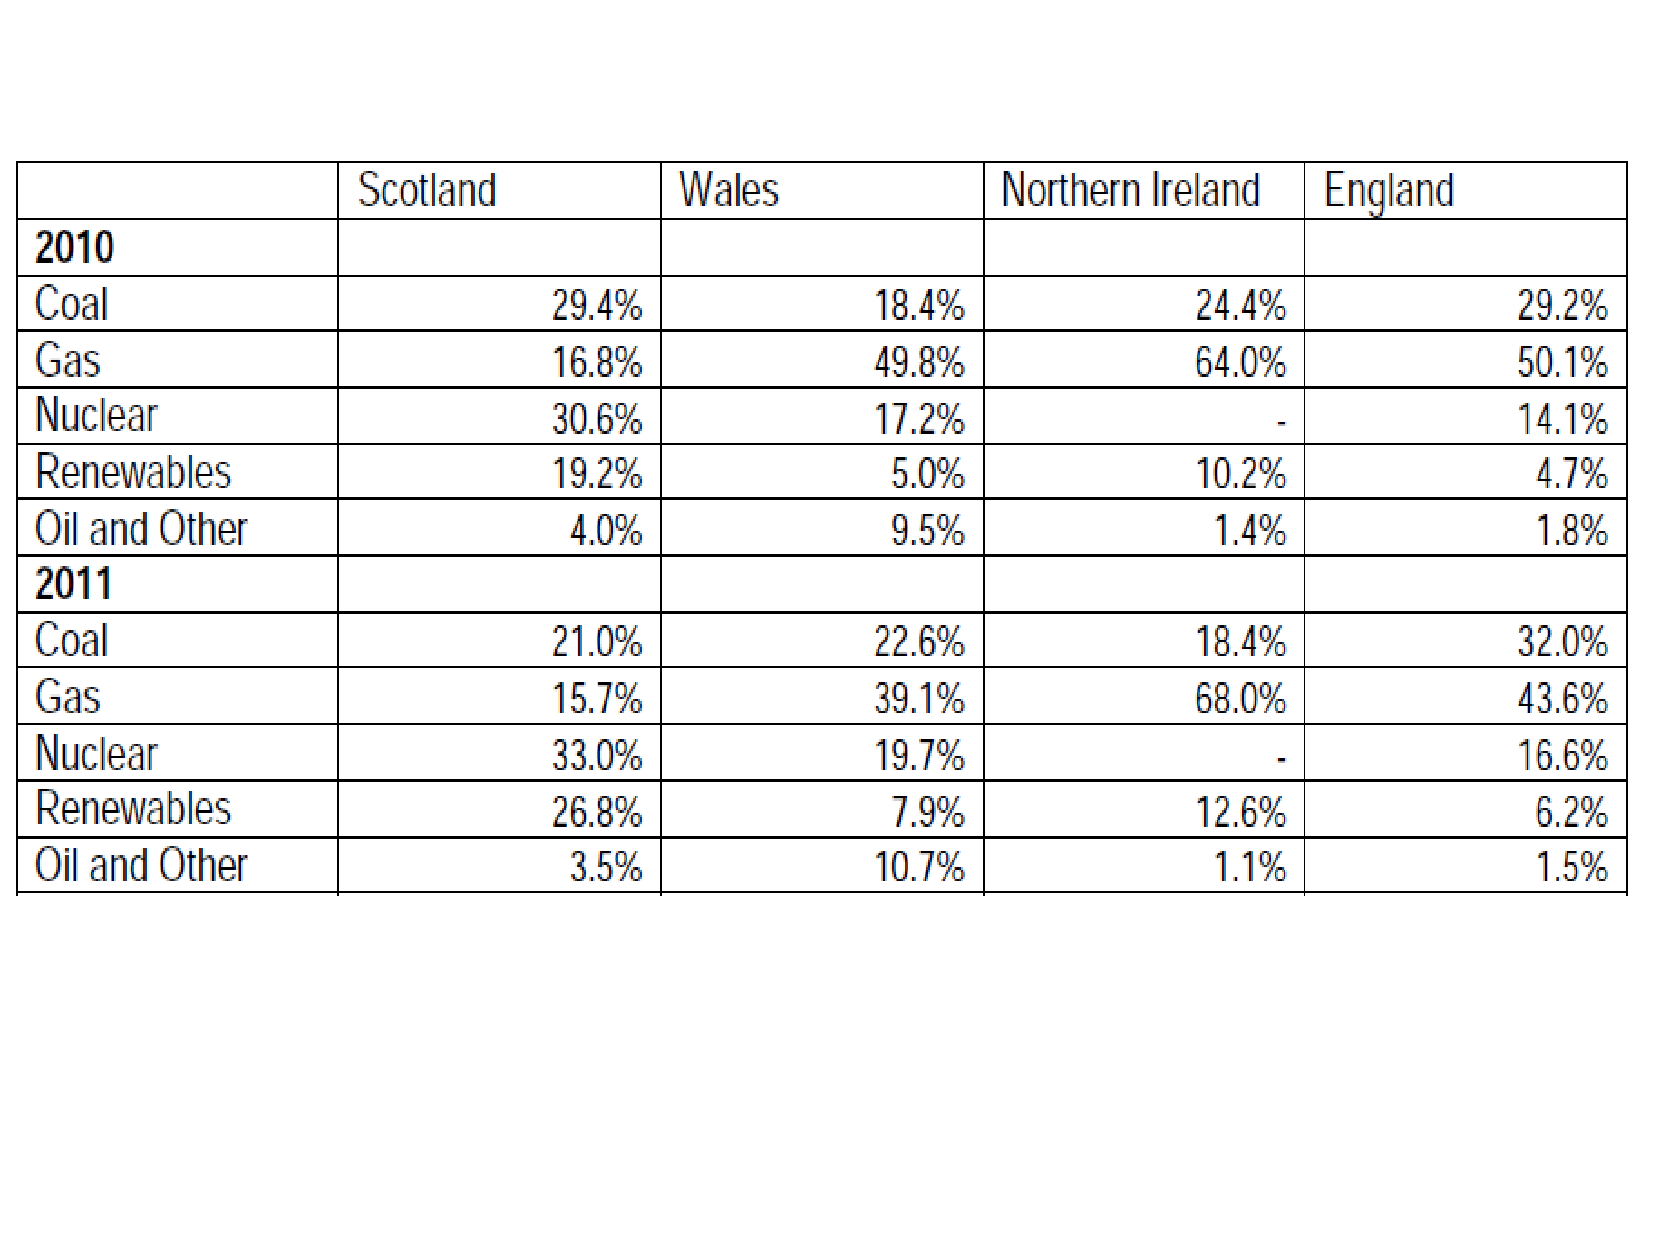
\includegraphics[width=9.cm,clip]{./Pics/Energy_Share_UK}
     \end{center}
    \end{figure}
\vspace{-2cm}
%\scriptsize
\textcolor{blue}{Fuel used in electricity generation and electricity supplied. (\href{https://www.gov.uk/government/organisations/department-of-energy-climate-change/series/electricity-statistics}{https://www.gov.uk/government/organisations/department-of-energy-climate-change/series/electricity-statistics})}
 \normalsize
\end{frame}


%%%
%%% Slide
%%%
\begin{frame}
 \frametitle{Introduction to Vapour and Gas Power}
    \begin{center}
     \begin{table}
       \begin{tabular}{l c c c}
    \hline
    \textcolor{blue}{Power Plant} & \textcolor{blue}{Renewable}  & \textcolor{blue}{Thermodynamic} \\
    \textcolor{blue}{Type}        & \textcolor{blue}{Source}     & \textcolor{blue}{Cycle}         \\
    \hline
      Coal                        &   No                         & Rankine  \\
      Natural Gas                 &   No                         & Brayton  \\
      Nuclear                     &   No                         & Rankine  \\
      Oil                         &   No                         & Rankine  \\
      Biomass                     &   Yes                        & Rankine  \\
      Geothermal                  &   Yes                        & Rankine  \\
      Solar ({\it Concentrated}   &   Yes                        & Rankine  \\
       {\it solar power)}         &                              &          \\
      Solar ({\it Photovoltaic})  &   No                         & None     \\
      Hydroelectric               &   Yes                        & None     \\
      Wind                        &   Yes                        & None     \\
      Currents, tides and         &   Yes                        & None     \\
      waves                       &                              &          \\
    %\hline
    %\hline
      \end{tabular}
     \end{table}
    \end{center}
\end{frame}

%%%
%%% Slide
%%%
\begin{frame}
 \frametitle{Introduction to Vapour and Gas Power}
 %\scriptsize
    \begin{enumerate}%\scriptsize
       \item<1-> While coal, natural gas, and nuclear still play important roles as energy sources, contributions from wind power, solar power, and other renewable sources are expected to be increasingly significant up to 2050;
       \item<2-> This table shows that thermodynamic cycles are crucial for a number of power plant types that employ renewable and non-renewable sources;
       \item<3-> The basic building block of vapour power systems is the \blue{Rankine cycle};
       \item<3-> Whereas gas power systems are based on \blue{Brayton cycles};
       \item <4-> Energy sources based on thermal-cycles (YouTube videos):
         \begin{itemize}%\scriptsize
            \item \href{http://www.youtube.com/watch?v=_UwexvaCMWA}{\textcolor{blue}{Nuclear Power Plants (NPP)}};
            \item \href{http://www.youtube.com/watch?v=0mjT8ETB128}{\textcolor{blue}{Coal-Fired Stations}};
            \item \href{http://www.youtube.com/watch?v=oi1TRbiE_Kw}{\textcolor{blue}{Gas Turbine Combined Cycle Power Plant}};
            \item \href{https://www.youtube.com/watch?v=kjpp2MQffnw}{\textcolor{blue}{Geothermal Power Plant}}.
         \end{itemize}
    \end{enumerate}
 \normalsize
\end{frame}

%%%
%%% SUBSECTION
%%%
\subsection{A Few Definitions}

%%%
%%% Slide
%%%
\begin{frame}
 \frametitle{A Few Definitions}
 %%\scriptsize
 \begin{itemize}
    \item<1-> A \blue{cycle} is defined as a repeated series of operations occurring in a certain order. A system is said to have undergone a cycle if it returns to its initial state at the end of the process.  Cycles can be classified as \red{ideal} (where there is no heat losses) and \red{real};
    \item<2-> In \blue{gas cycles}, the working fluid remains in the gas phase throughout the cycle (e.g., air);
    \item<3-> In \blue{vapour cycles}, the working fluid exists as a vapour for part of the cycle and liquid for the other part -- i.e., the working fluid is alternately \red{vaporised and condensed};
    \item<4-> \blue{Water steam} is the most common working fluid in vapour power cycles as it has many desirable characteristics: low cost, availability and high enthalpy of vaporisation;
    %\item<5-> Coal, nuclear, natural gas and geothermal power plants are examples of steam power plants. Each utilises a different type of fuel to supply heat to the steam cycle;
    \item<5-> In \blue{closed cycles}, after each pass through the cycle the working fluid remains within the system;
    \item<6-> In \blue{open cycles}, after a few (or a single) pass through the cycle the working fluid is replaced by a fresh working fluid.
 \end{itemize}
 %\normalsize
\end{frame}


%%%
%%% Slide
%%%
\begin{frame}
 \frametitle{A Few Definitions -- Open Cycles}
 \scriptsize
 \begin{columns}
  \begin{column}[c]{0.5\linewidth}
   \visible<1->{\begin{figure}%
    \begin{center}
     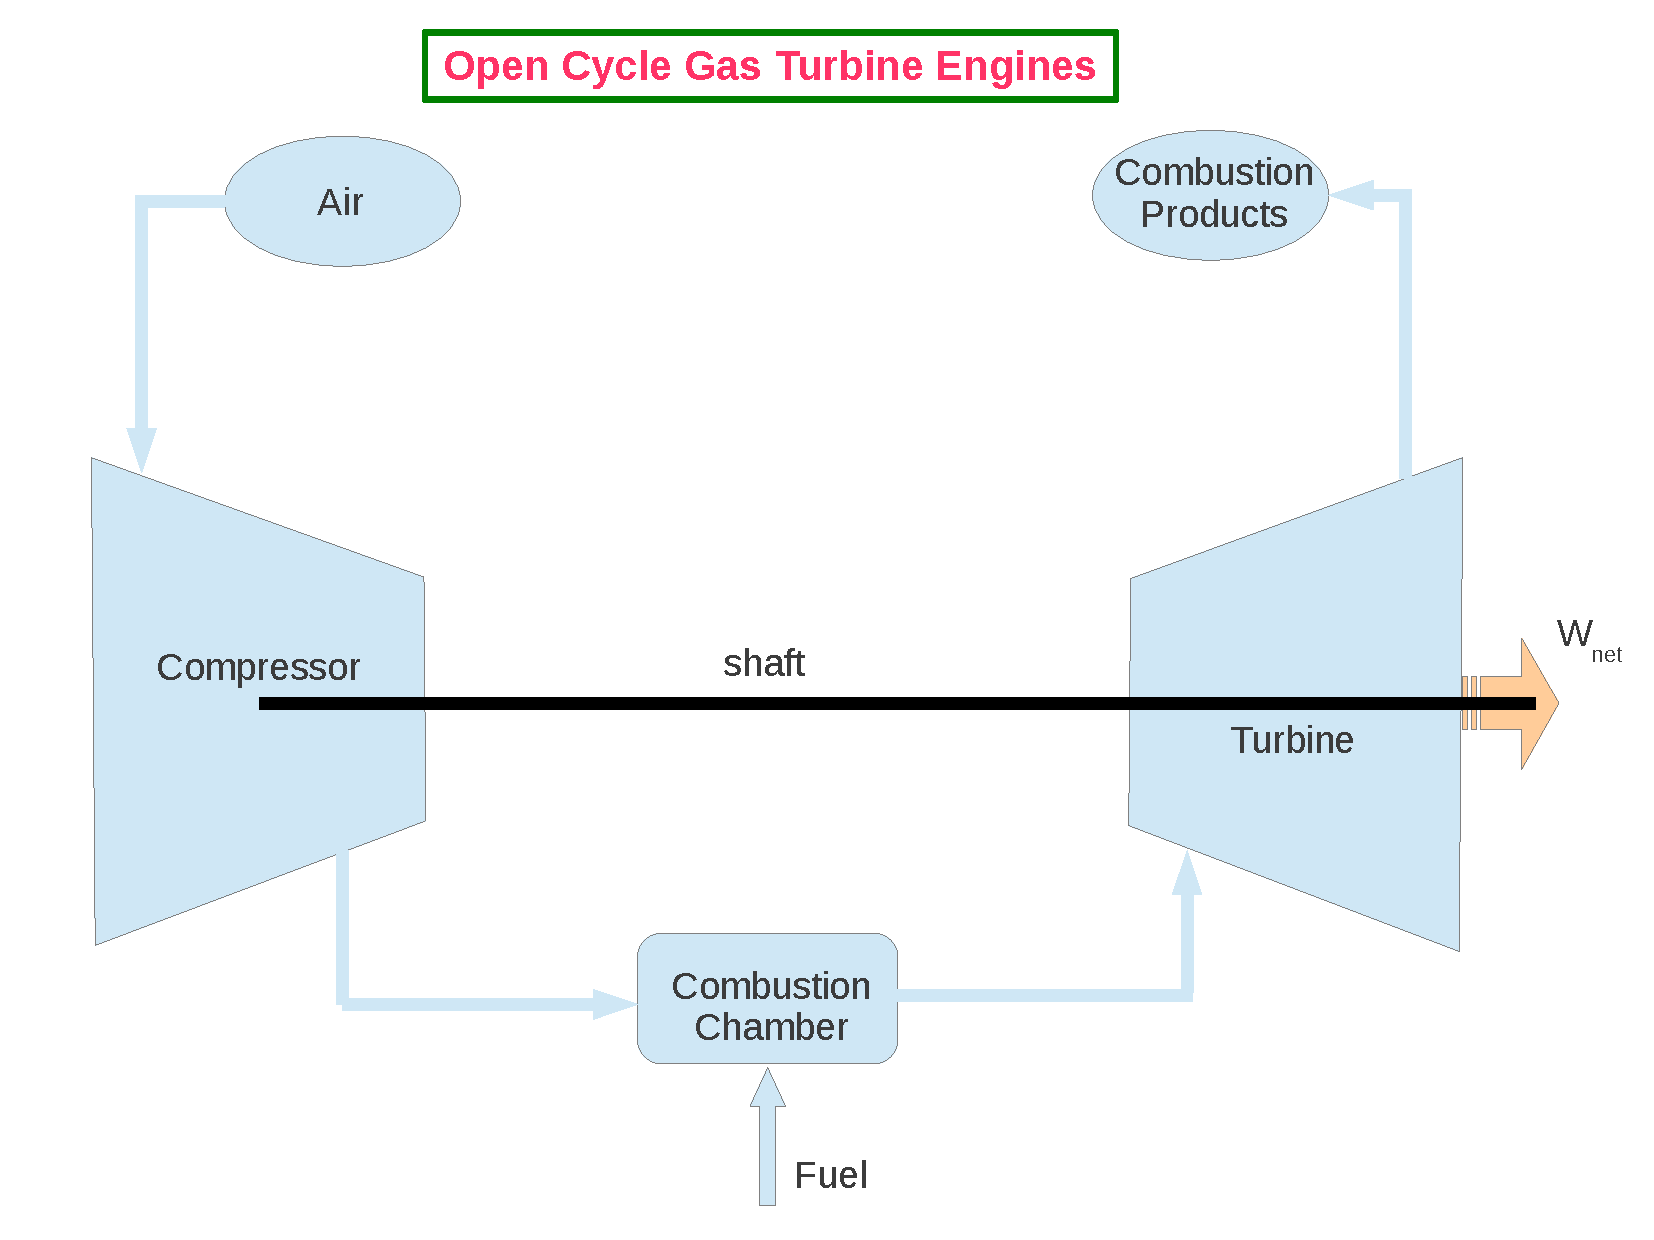
\includegraphics[width=6.2cm,clip]{./Pics/Open_Gas_Turbine_Engines}
    \end{center}
   \end{figure}} \vspace{-.5cm}
     \begin{enumerate}[(i)]\scriptsize
      \item<2-> \blue{Isentropic} (reversible adiabatic) \blue{compression};
      \item<3-> \blue{Constant pressure heat supply} in the combustion chamber;
      \item<4-> \blue{Isentropic} (reversible adiabatic) \blue{expansion} of combustion gases;
      \item<5-> Combustion products (CO$_{2}$, CO, H$_{2}$O, etc) are exhausted into the atmosphere.
     \end{enumerate}
  \end{column}  
  \begin{column}[c]{0.5\linewidth}
   \visible<6->{\begin{figure}%
    \begin{center}
     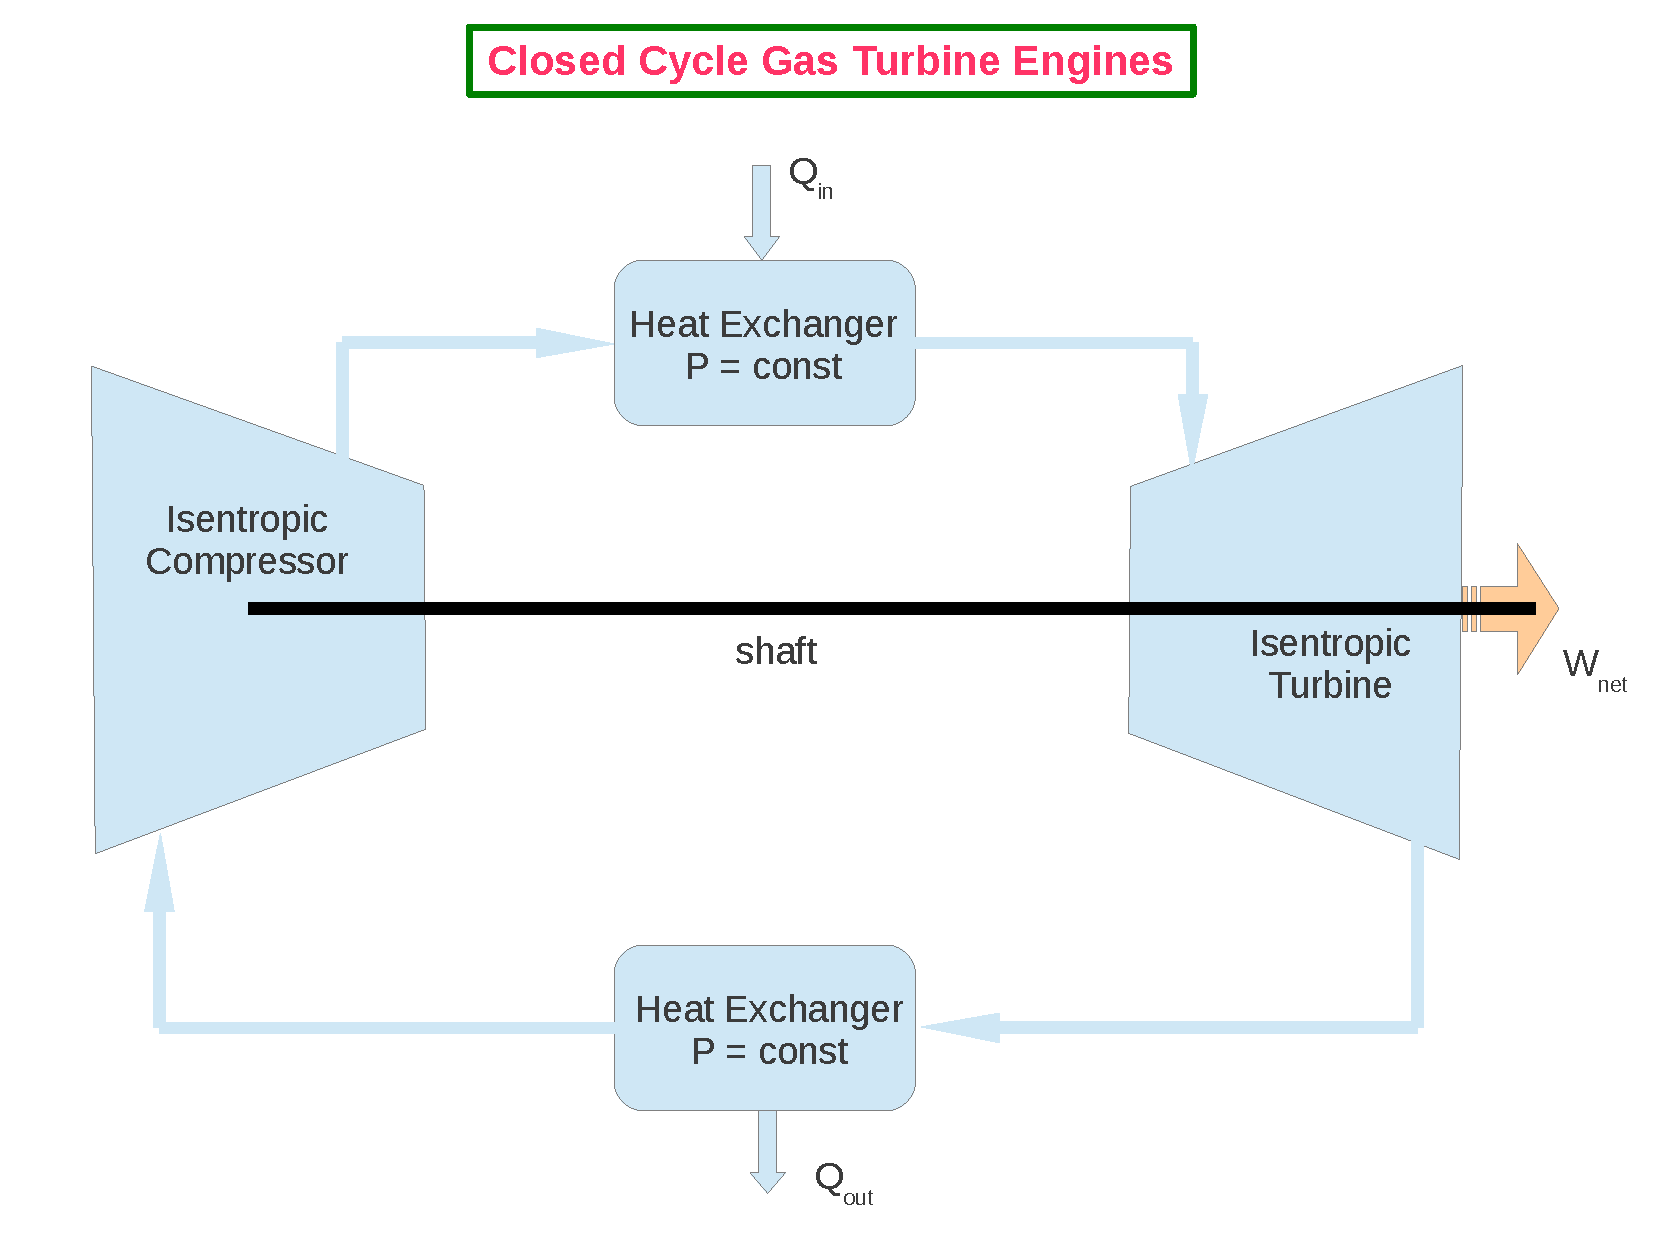
\includegraphics[width=6.2cm,clip]{./Pics/Closed_Gas_Turbine_Engines}
    \end{center}
   \end{figure}}   \vspace{-.5cm}
     \begin{enumerate}[(i)]\scriptsize
       \item <7-> It comprises a compressor, air heater, turbine and a cooler;
       \item <8-> Fuel is burnt externally and heat is supplied to working substance (fluid) in the heater;
       \item <9-> It uses an external combustion turbine;
     \end{enumerate}
  \end{column}  
 \end{columns}
 \normalsize
\end{frame}


%%%
%%% SECTION
%%% 
\section{Vapour Power System}

\subsection{Carnot Engines and Carnot Cycle}

%%%
%%% Slide
%%%
\begin{frame}
 %\scriptsize
 \frametitle{The Carnot Cycle}
  \begin{columns}
   \begin{column}[c]{0.6\linewidth}
    \begin{enumerate}[(a)] \scriptsize
     \item <1-> A \blue{heat engine} is a closed system that converts heat to work and operates in a cycle;
     \item <2-> A \blue{Carnot cycle} has four reversible steps, alternating isothermal (and isobaric: 4-1, 2-3) and frictionless adiabatic (i.e., \blue{isentropic}, 1-2, 3-4):
       \begin{enumerate}[(i)]\scriptsize
         \item <3-> {\it Step 1-2}: \blue{Steam} is \red{isentropically} expanded to $T_{2}$ and $P_{2}$;
         \item <4-> {\it Step 2-3}: Heat is rejected at \red{constant pressure} $\left(P_{2}\right)$ \red{and temperature} $\left(T_{2}\right)$. During this step, steam becomes wetter and cooled;
         \item <5-> {\it Step 3-4}: Wet steam is \red{isentropically} compressed until the steam returns to its original state at $T_{1}$ and $P_{1}$ (saturated liquid);
         \item <6-> {\it Step 4-1}: \blue{Boiling water} at temperature $T_{1}$ is heated to form wet steam $\left(\right.$dryness fraction $x_{1}\left.\right)$. Heat is then absorbed at \red{constant temperature} $\left(T_{1}\right)$ \red{and pressure} $\left(P_{1}\right)$;
       \end{enumerate}
     \item <7-> The efficiency of the \blue{Carnot cycle} is given by:
          \visible<7->{\begin{equation}
             \blue{\eta_{\text{Carnot}}} = \frc{\text{Work Done}}{\text{Heat Supplied}} \blue{= 1 - \frc{T_{2}}{T_{1}}}
          \end{equation}}
    \end{enumerate} 
   \end{column}
   \begin{column}[c]{0.4\linewidth}
   \begin{figure}%
    \begin{center}
     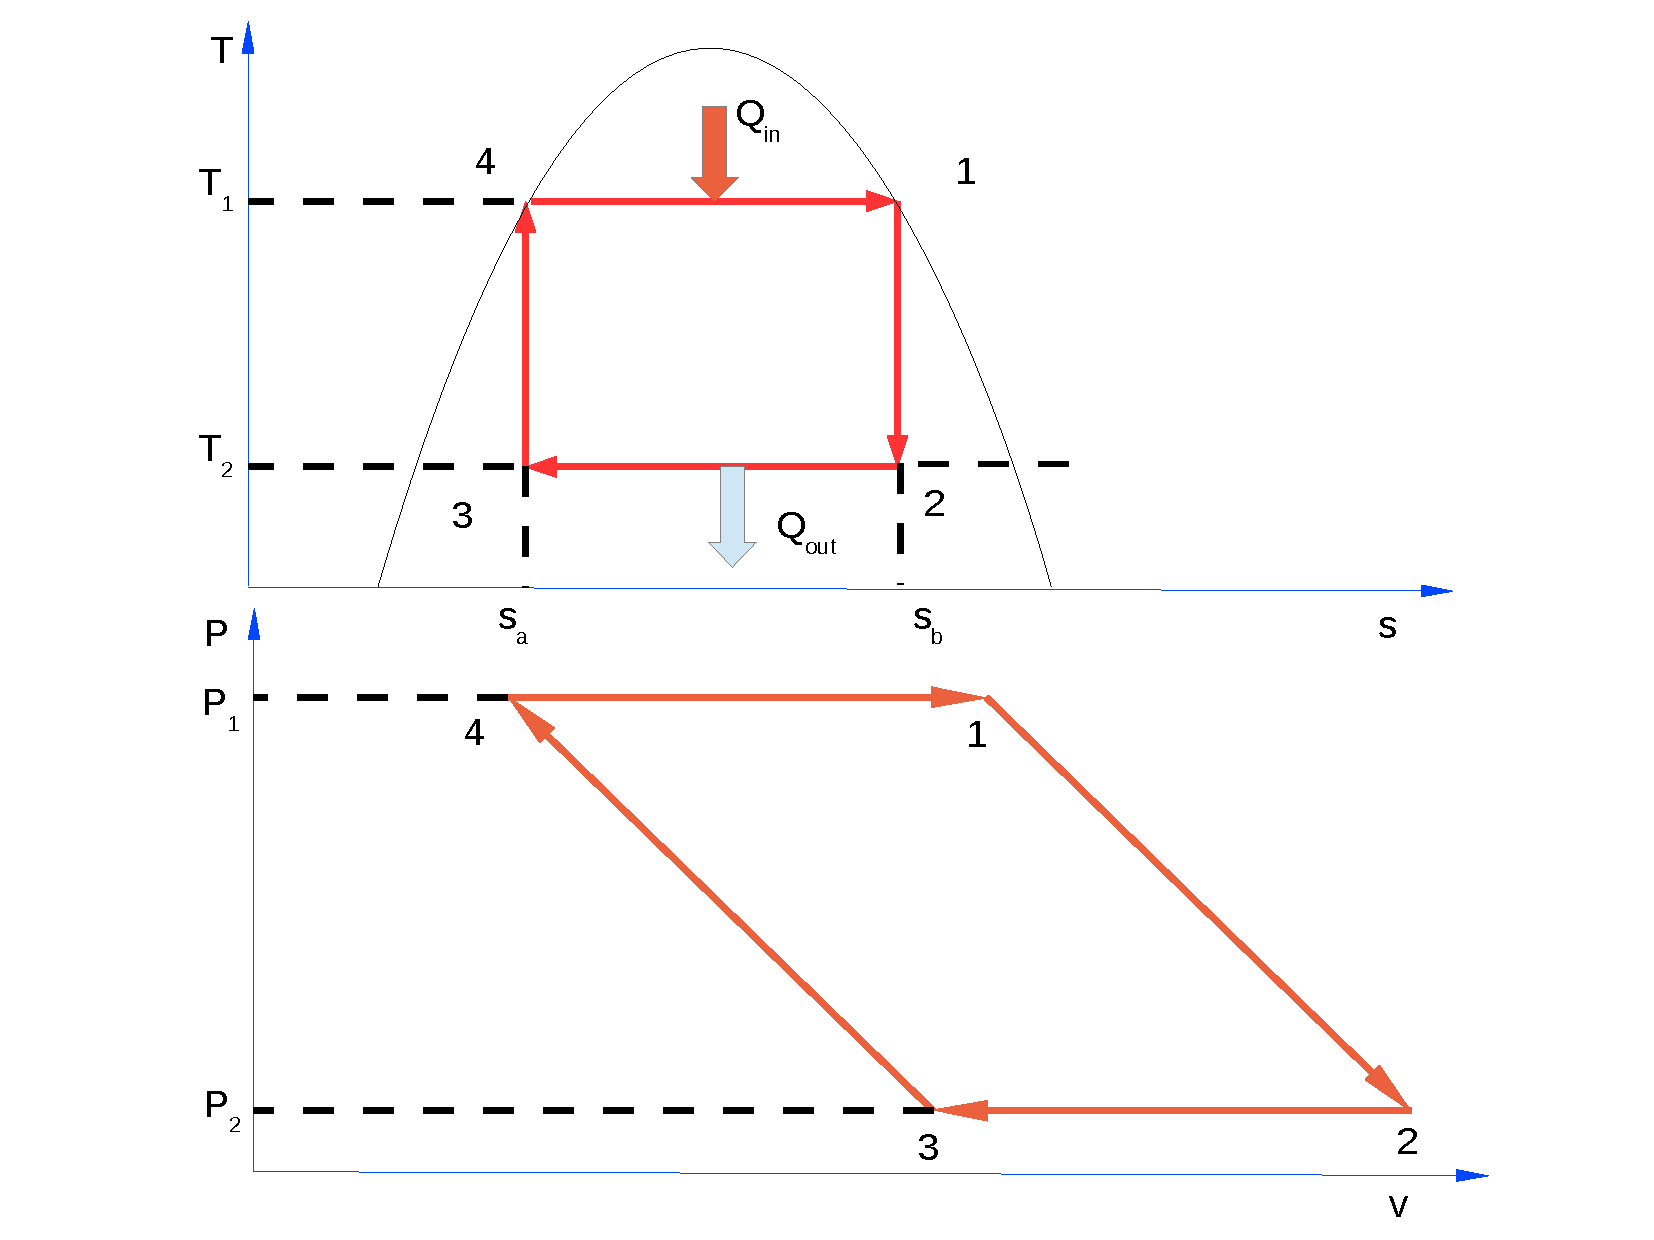
\includegraphics[width=5.5cm,clip]{./Pics/Carnot_PV_TS}
    \end{center}
   \end{figure}    
   \end{column}
  \end{columns}
 \normalsize
\end{frame}

%%%
%%% Slide
%%%
\begin{frame}
 \frametitle{Limitations of the Carnot Cycle}
 %\scriptsize
 \begin{enumerate}[(a)]
  \item <1-> The \blue{Carnot cycle} is thermodynamically simple and has the \red{highest thermal efficiency} for a given temperature gradient;
  \item <2-> It is however {\it difficult to operate in practice} due to:
  \begin{enumerate}[(i)] %\scriptsize
   \item <3-> It is difficult to compress a wet vapour isentropically to the saturated state (as required by the process 3-4);
   \item <4-> It is difficult to control the quality of the condensate produced by the condenser to reach state 3;
   \item <5-> The efficiency is greatly affected by $T_{1}$ at which heat is transferred to the working fluid. As the critical temperature of steam is 374$^{\circ}$C therefore, if the cycle is to be operated in the wet region, the maximum possible temperature is severely limited;
   \item <6-> The cycle is even more difficult to operate in practice with superheated steam due to the necessity to supply superheated steam at constant temperature instead of constant pressure (as it is usual in industrial plants);
   \item <7-> \textcolor{blue}{{\it In a practical cycle, limits of pressure and volume are easier to be obtained than limits of temperature. Therefore no practical engine operates in the Carnot cycle, although all modern cycles aspire to achieve it.}}
  \end{enumerate}
 \end{enumerate}
 \normalsize
\end{frame}

%%%
%%% SUBSECTION
%%%
\subsection{The Rankine Cycle}

%%%
%%% Slide
%%%
\begin{frame}
 \frametitle{Rankine Cycle}
 %\scriptsize
 \begin{columns}
   \begin{column}[c]{0.5\linewidth}
    \begin{figure}%
     \begin{center}
      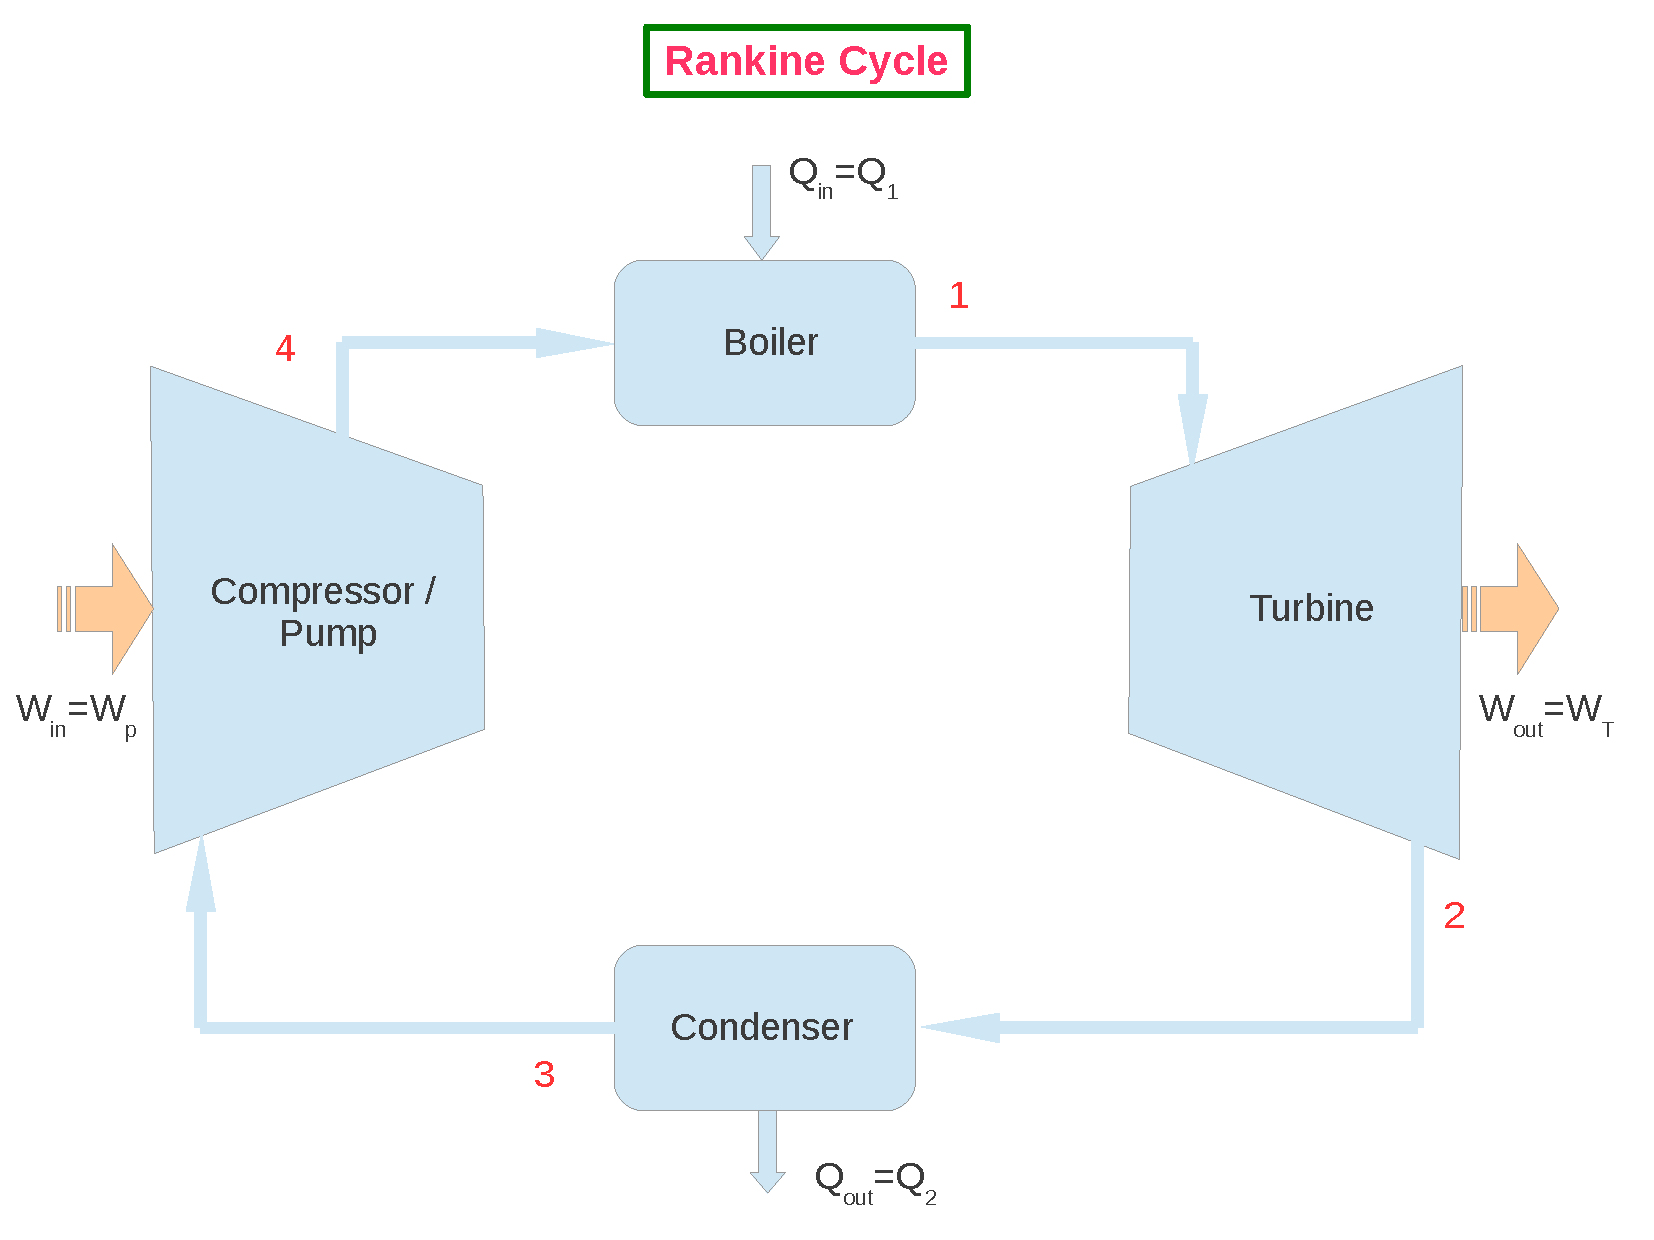
\includegraphics[width=6.5cm,clip]{./Pics/Simple_Rankine_Cycle}
     \end{center}
    \end{figure}  
   \end{column}
   \begin{column}[l]{0.5\linewidth}
    \begin{enumerate}[(a)]\scriptsize
     \item<1->\textcolor{blue}{Rankine Cycle} (RC) is the ideal cycle for vapour power plants;
     \item<2-> It does not involve any internal irreversibilities and consists of the following four processes:
     \begin{enumerate}[(i)]\scriptsize
      \item<3-> \textcolor{red}{Process 1-2}: reversible adiabatic (i.e., \blue{isentropic}) expansion in the turbine (or steam engine);
      \item<4-> \textcolor{red}{Process 2-3}: constant-pressure heat transfer in the condenser;
      \item<5-> \textcolor{red}{Process 3-4}: reversible adiabatic (i.e., \blue{isentropic}) pumping process in the feed pump;
      \item<6-> \textcolor{red}{Process 4-1}: constant-pressure heat transfer in the boiler.  
     \end{enumerate}
     \item<7-> Efficiency of the \blue{RC} can be expressed as:
       \visible<7->{\begin{eqnarray}
          \blue{\eta_{\text{Rankine}}} &=& \frc{W_{\text{net}}}{Q_{1}} = \frc{W_{T}-W_{P}}{Q_{1}}\nonumber \\
                                    &=& \frc{\left(h_{1}-h_{2}\right)-\left(h_{f4}-h_{f3}\right)}{h_{1}-h_{f4}} \nonumber \\
                                    &=& \blue{\frc{h_{1}-h_{2}}{h_{1}-h_{f4}}} 
       \end{eqnarray}}
    \end{enumerate}
   \end{column}
  \end{columns}
 \normalsize
\end{frame}


%%%
%%% Slide
%%%
\begin{frame}
 \frametitle{Rankine Cycle: {\it Pv}, {\it Ts} and {\it hs} Diagrams}
 %\scriptsize
 \begin{columns}
%
   \begin{column}[l]{0.45\linewidth}
    \begin{figure}%
     \begin{center}
      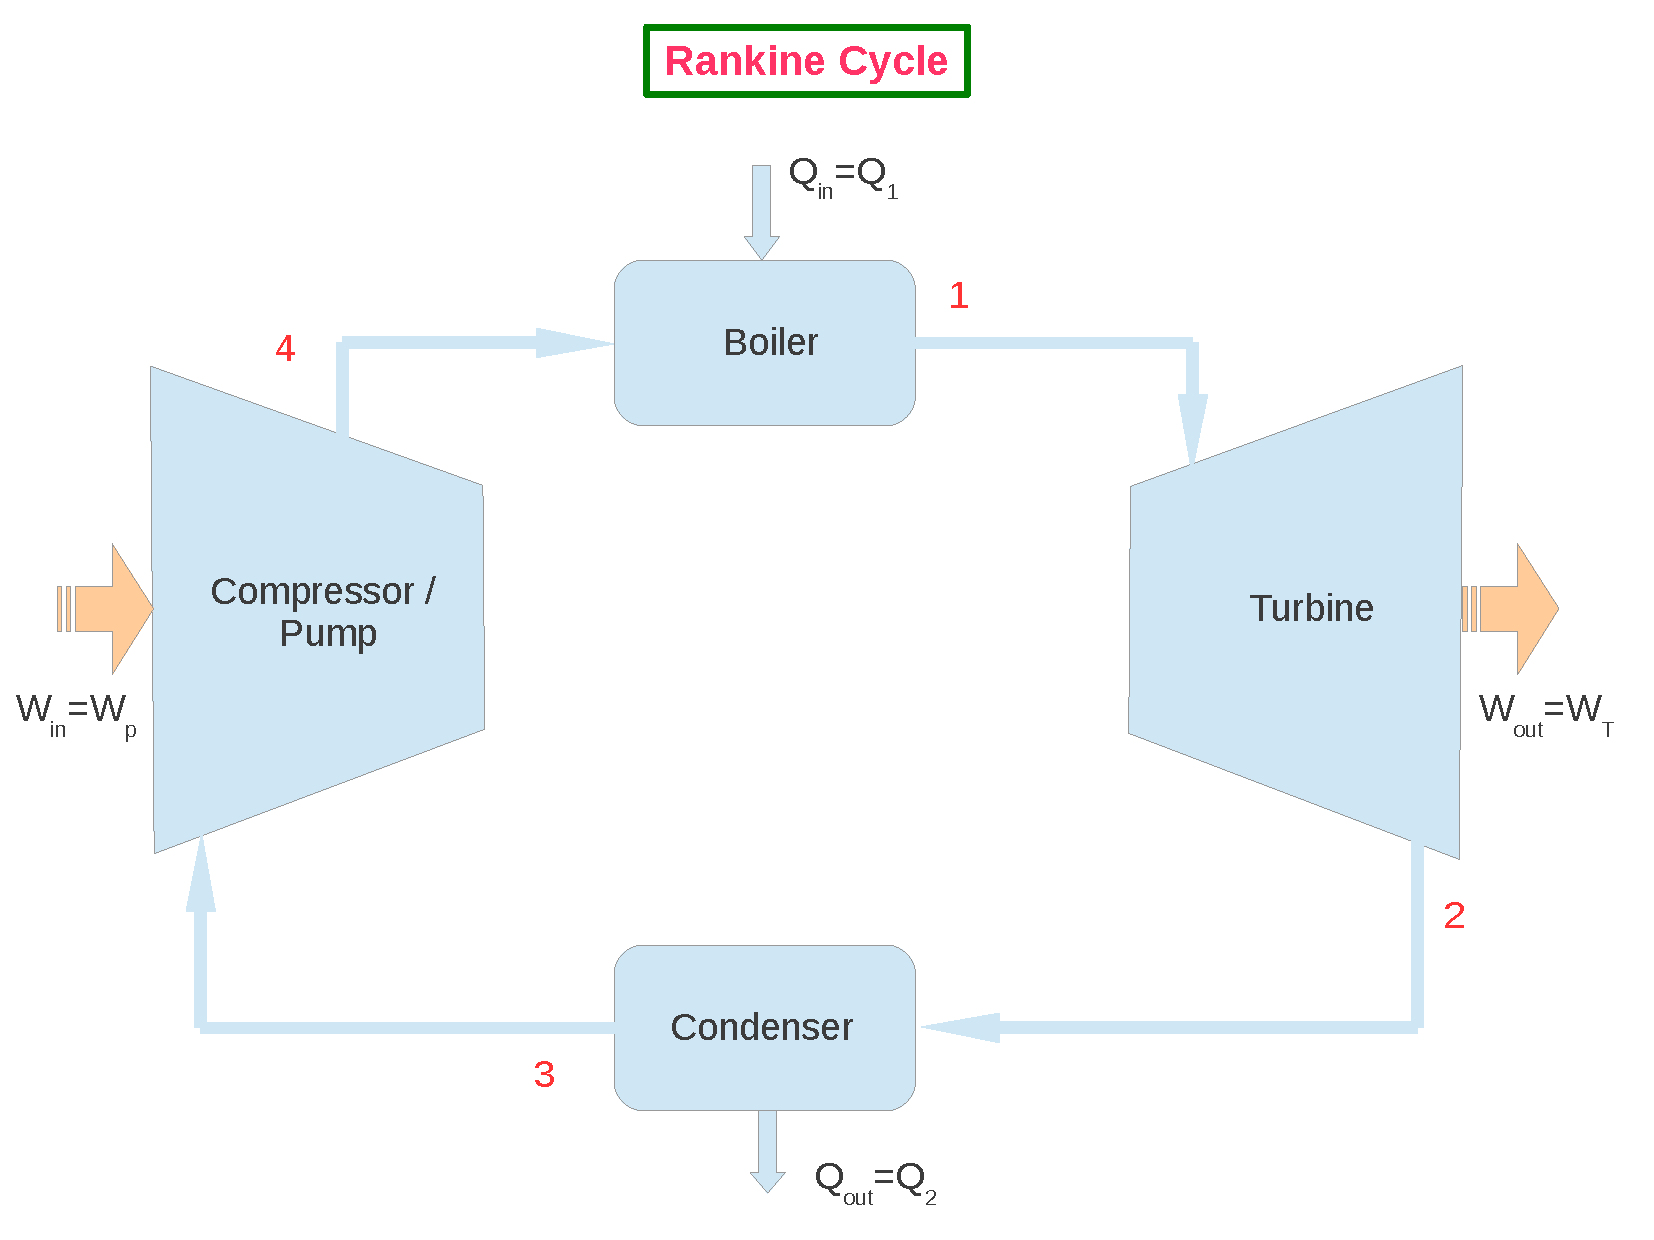
\includegraphics[width=5.5cm,clip]{./Pics/Simple_Rankine_Cycle}
     \end{center}
    \end{figure} 
    \begin{block}{\begin{center}Quality of the Vapour\end{center}}
       \begin{equation}\scriptsize
         \blue{x_{j} = \frc{\Psi_{j}-\Psi_{f}}{\Psi_{g}-\Psi_{f}}} \;\;\;\text{with }\Psi=\left\{h,s\right\}
       \end{equation}
    \end{block}
   \end{column}
%
   \begin{column}[c]{0.55\linewidth}
    \begin{figure}%
     \begin{center}
      \visible<2->{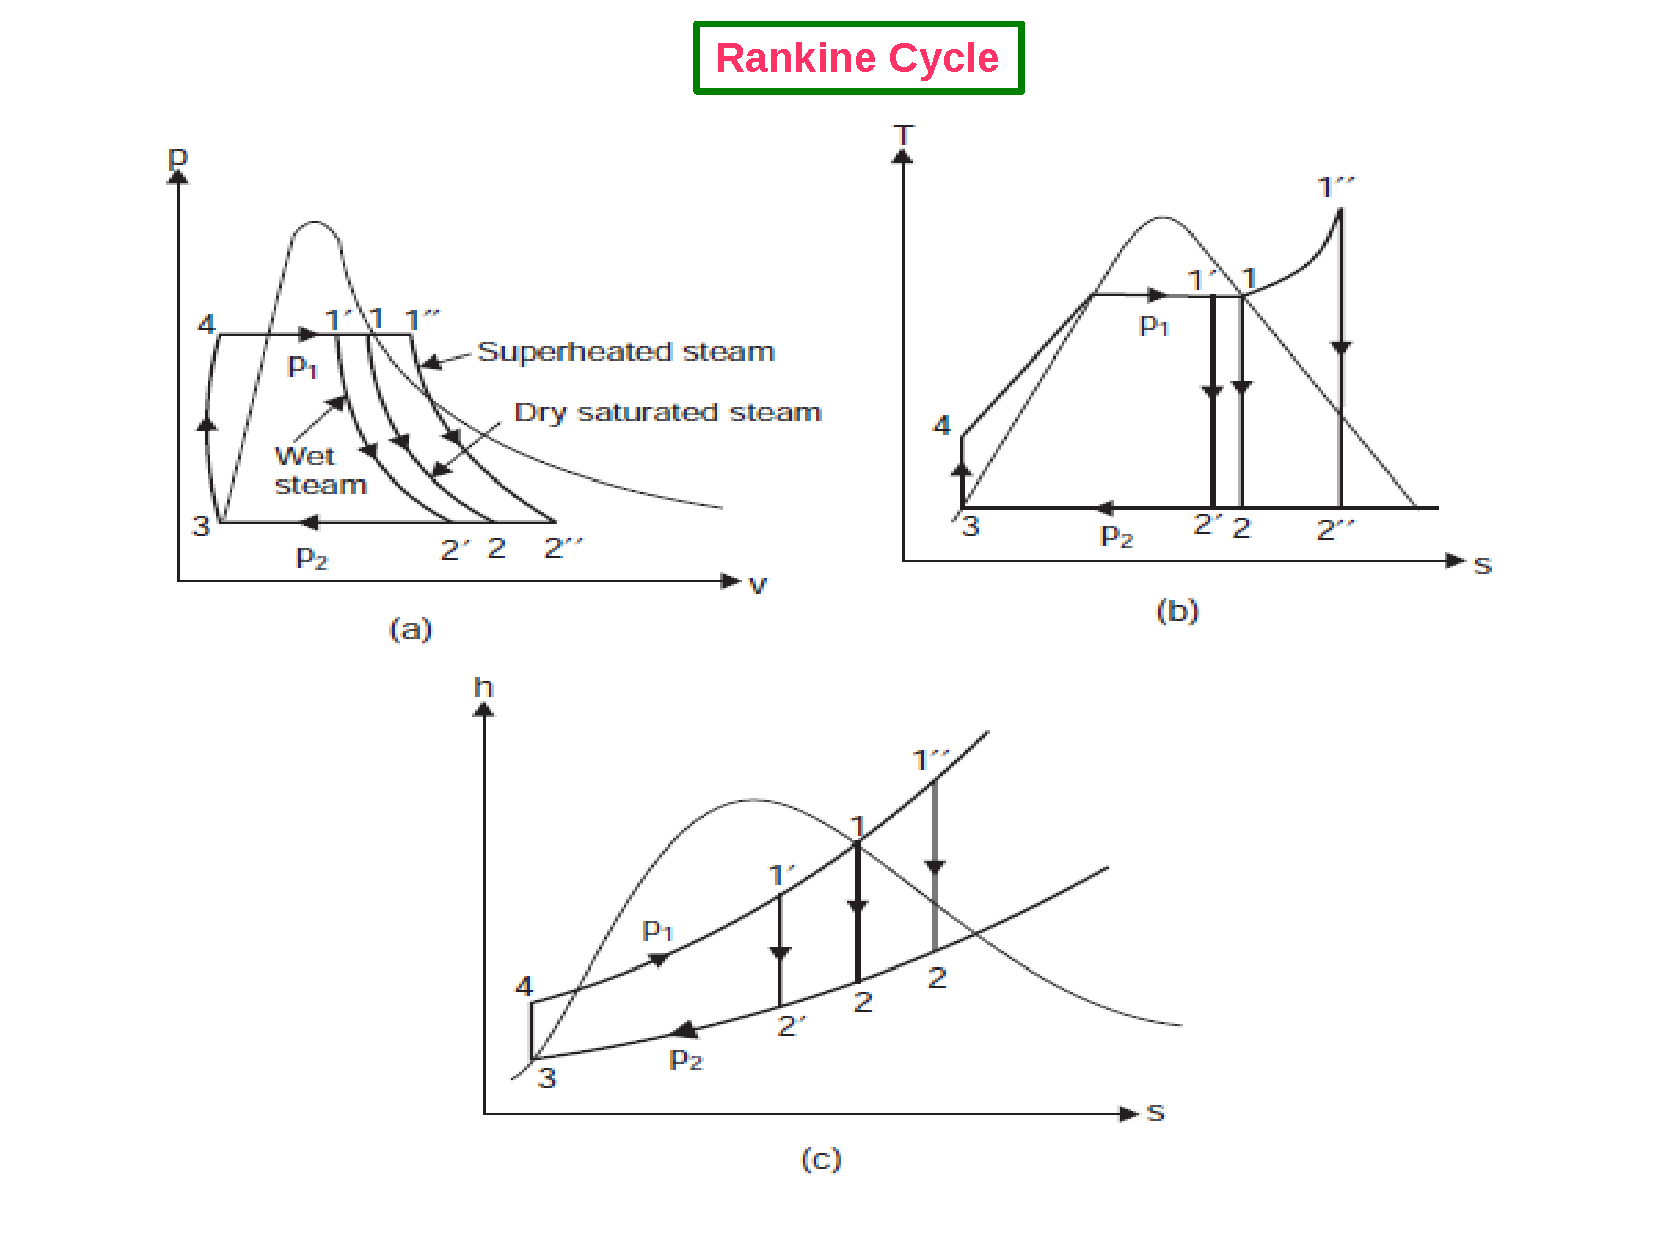
\includegraphics[width=7.5cm,clip]{./Pics/Simple_Rankine_Cycle_Diagrams}}
     \end{center}
    \end{figure}  
   \end{column}
  \end{columns}
\end{frame}


%%%
%%% Slide
%%%
\begin{frame}
 \frametitle{Comparison between Rankine and Carnot Cycles}
 %\scriptsize
  \begin{columns}
   \begin{column}[c]{0.4\linewidth}
    \begin{enumerate}[(a)]\scriptsize
     \item<1-> Between the same temperature range $\left(T_{1}\text{ and }T_{2}\right)$, \blue{RC} provides higher specific work output than Carnot cycles $\Longrightarrow$ \red{RC requires a smaller steam flow rate};
     \item<2-> However, \blue{RC requires larger heat transfer rates between the boiler and the condenser};
     \item<3-> Also, only part of the heat is supplied \blue{isothermally at constant high temperature $T_{1}$}, therefore \blue{the efficiency is lower than that of Carnot cycle}. The efficiency of the \blue{RC} will approach that of the Carnot cycle more nearly if the superheat temperature rise is reduced;
     \item<4-> \red{The advantage of using pump to feed liquid to the boiler instead to compressing a wet vapour is because the work for steam compression is larger than pumping liquid}.
    \end{enumerate}
   \end{column}
   \begin{column}[c]{0.6\linewidth}
    \begin{figure}%
     \begin{center}
      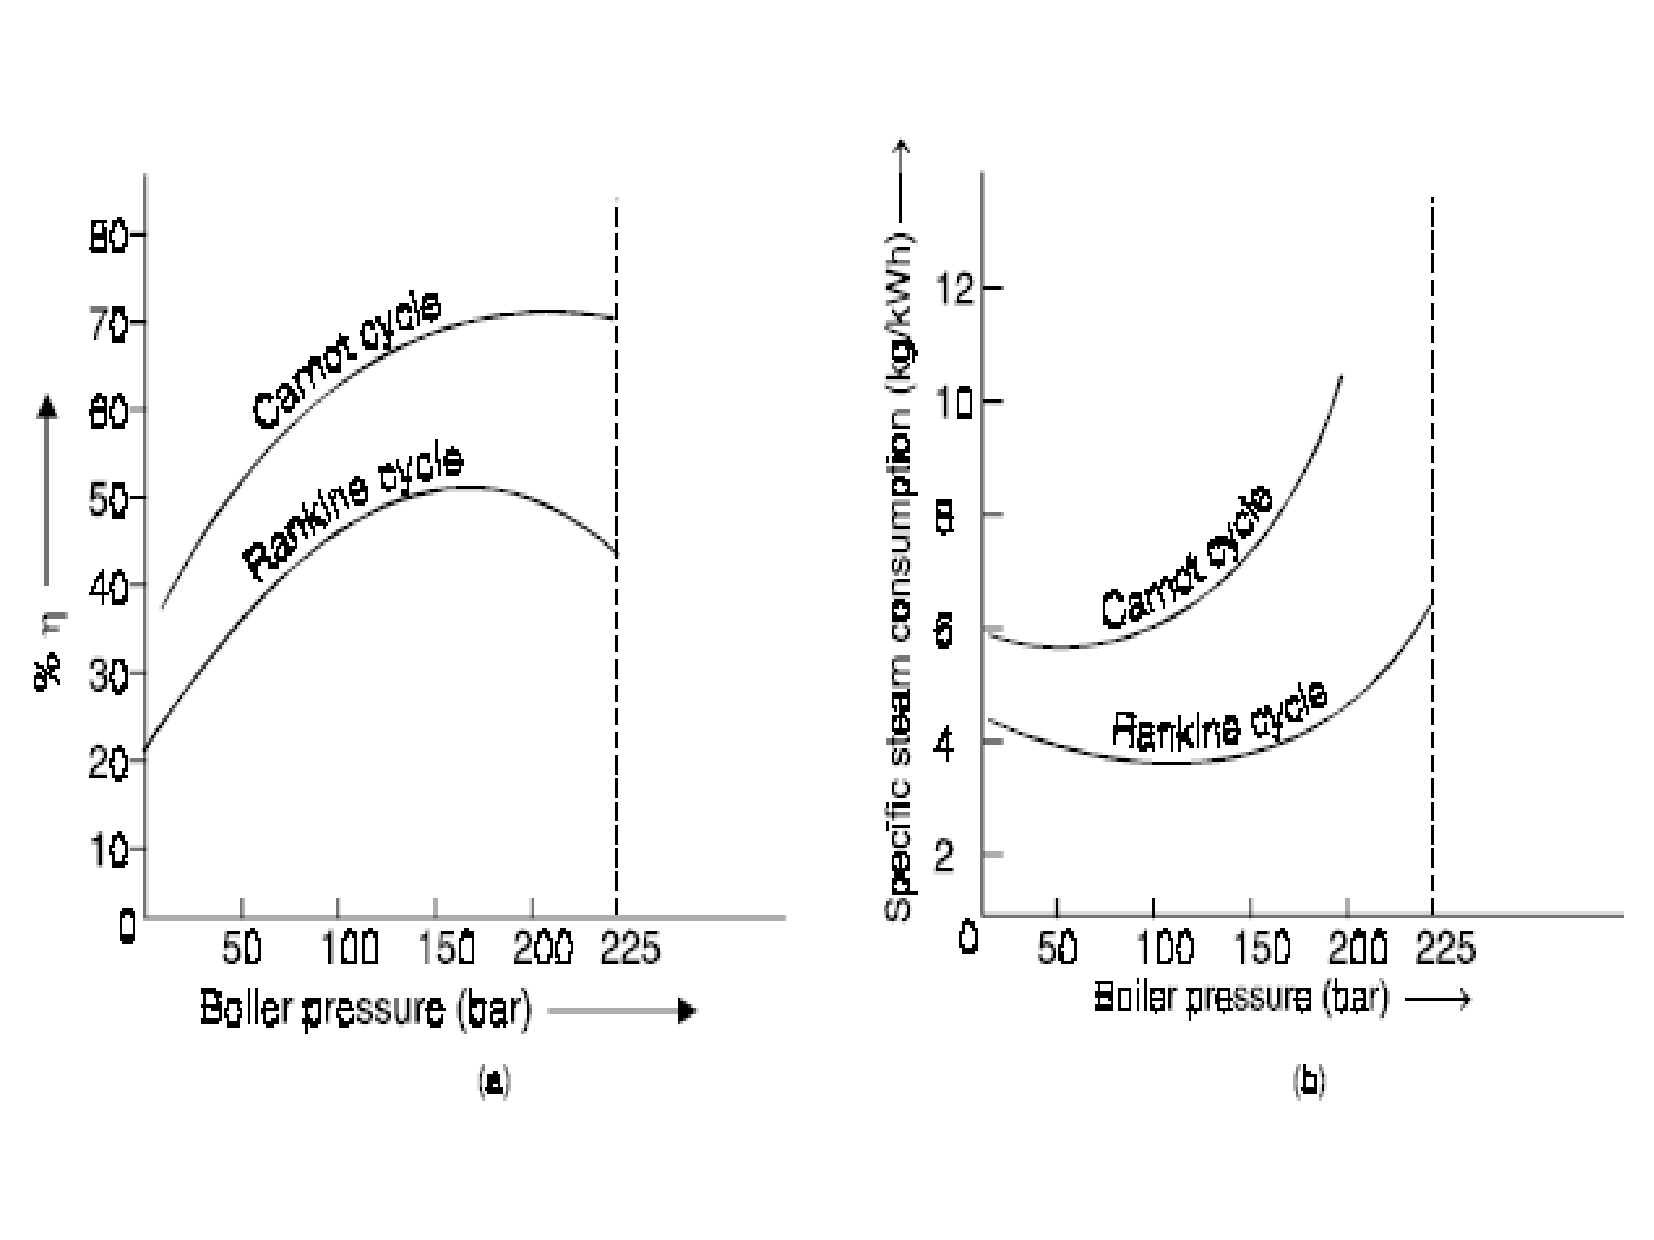
\includegraphics[width=7.5cm,clip]{./Pics/Comparison_Rankine_Carnot}
     \end{center}
    \end{figure}  
   \end{column}
  \end{columns}
 \normalsize
\end{frame}


%%%
%%% Slide
%%%
\begin{frame}
 \frametitle{Ideal {\it versus} Actual Rankine Cycles}
   \begin{columns}
      \begin{column}[c]{0.5\linewidth}
         \begin{enumerate}\scriptsize
             \item<1-> Differences between actual and ideal RC are mainly due to \blue{fluid friction} resulting in \blue{pressure drop in the boiler, condenser and pipes};
             \item<2-> Steam leaves the boiler at a pressure lower than expected; 
             \item<3-> \underline{Fluid pressure at the turbine inlet} is also \underline{lower than that at the boiler exit} due to pressure drop between pipes; 
             \item<4-> Pressure drop in the \blue{condenser} is usually \underline{negligible}; 
             \item<5-> In order to mitigate these pressure drops throughout power cycles, water must be pumped to a pressure higher than the required in the ideal cycle. Thus, a more powerful pump (and therefore larger worker input to the pump) is needed, increasing the energy cost.  
         \end{enumerate}\scriptsize
         \visible<6->{\begin{block}{\begin{center}Efficiencies of Turbines and Pumps\end{center}}
           \begin{eqnarray}\scriptsize
              && \blue{\eta_{T}=} \frc{W_{T,a}}{W_{T,s}} = \blue{\frc{h_{2}-h_{1}}{h_{2s}-h_{1}}} \\
              && \blue{\eta_{P}=} \frc{W_{P,s}}{W_{P,a}} = \blue{\frc{h_{4s}-h_{3}}{h_{4}-h_{3}}}
           \end{eqnarray}
         \end{block}}
      \end{column}
      \begin{column}[c]{0.5\linewidth}
         \vbox{
           \hbox{\hspace{.5cm}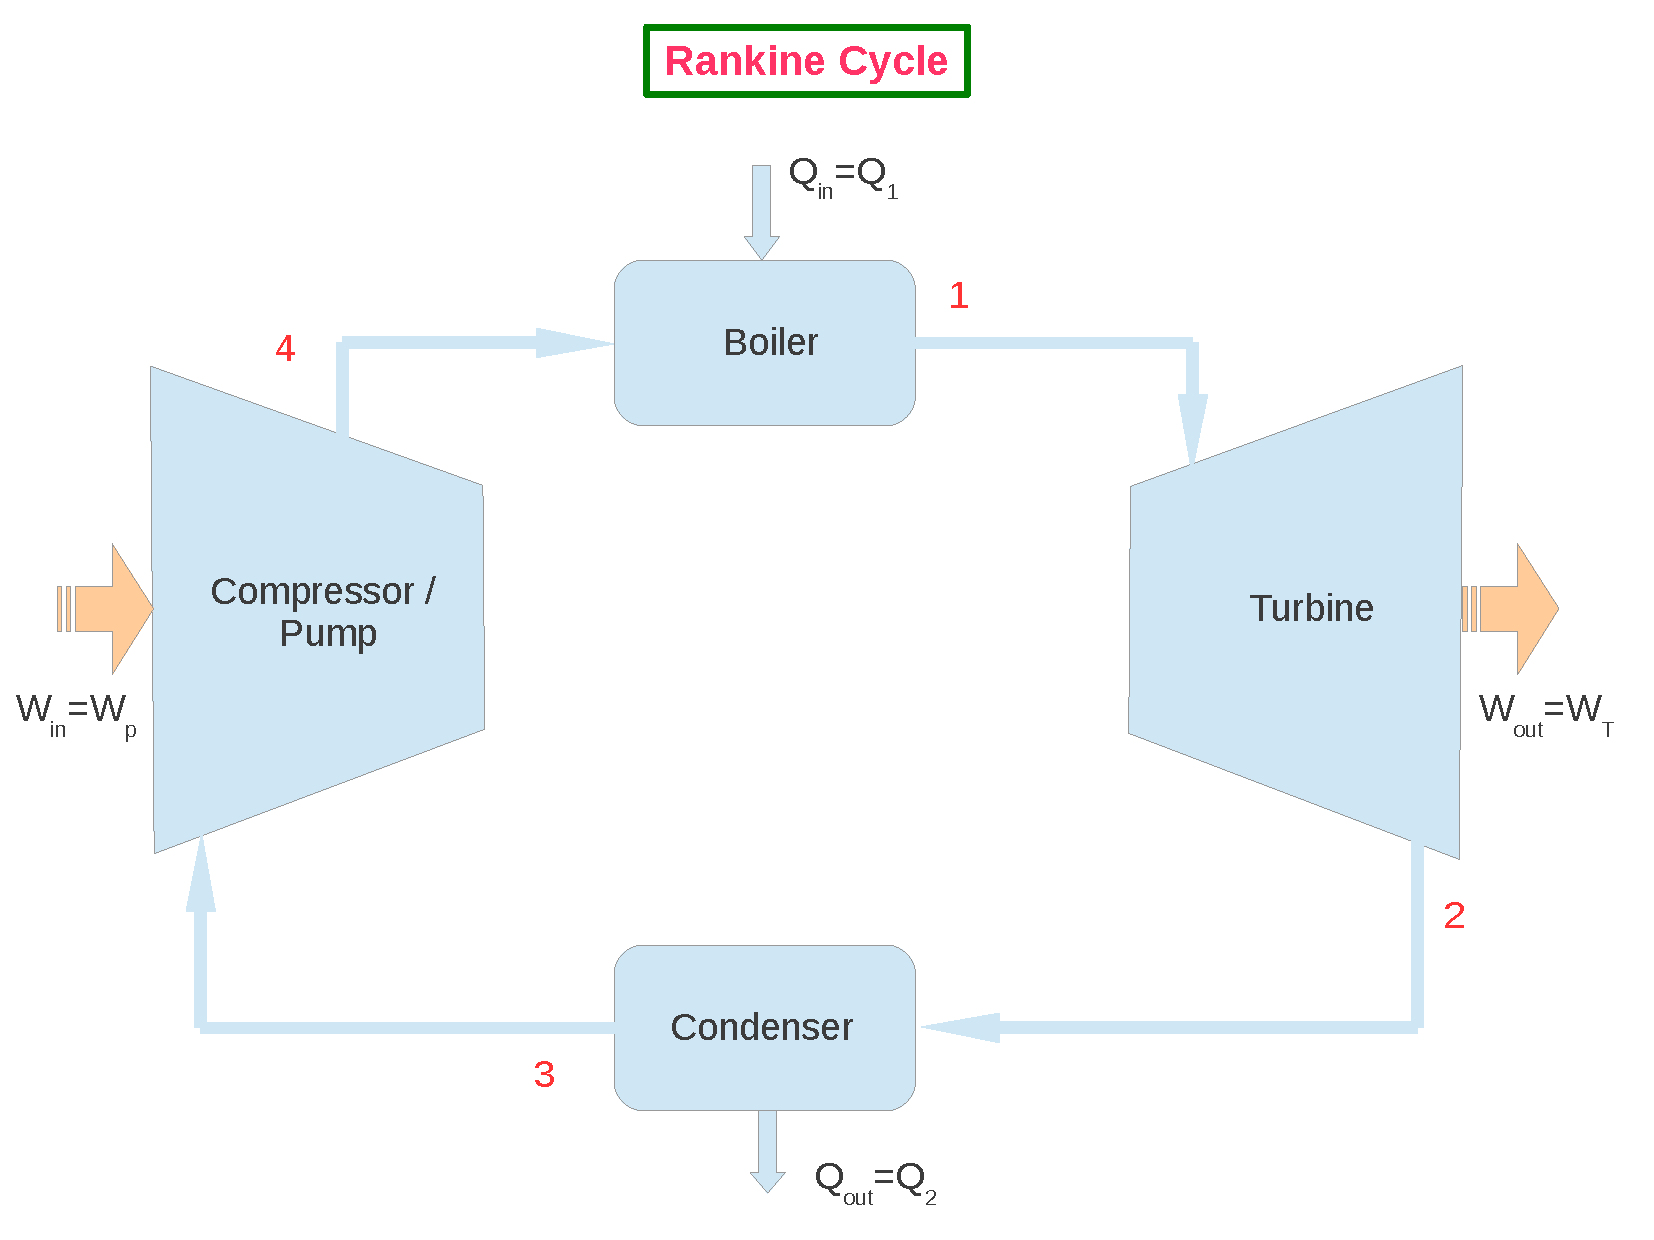
\includegraphics[width=5.cm,clip]{./Pics/Simple_Rankine_Cycle}}
           \vspace{-0.1cm}
           \hbox{\hspace{.5cm}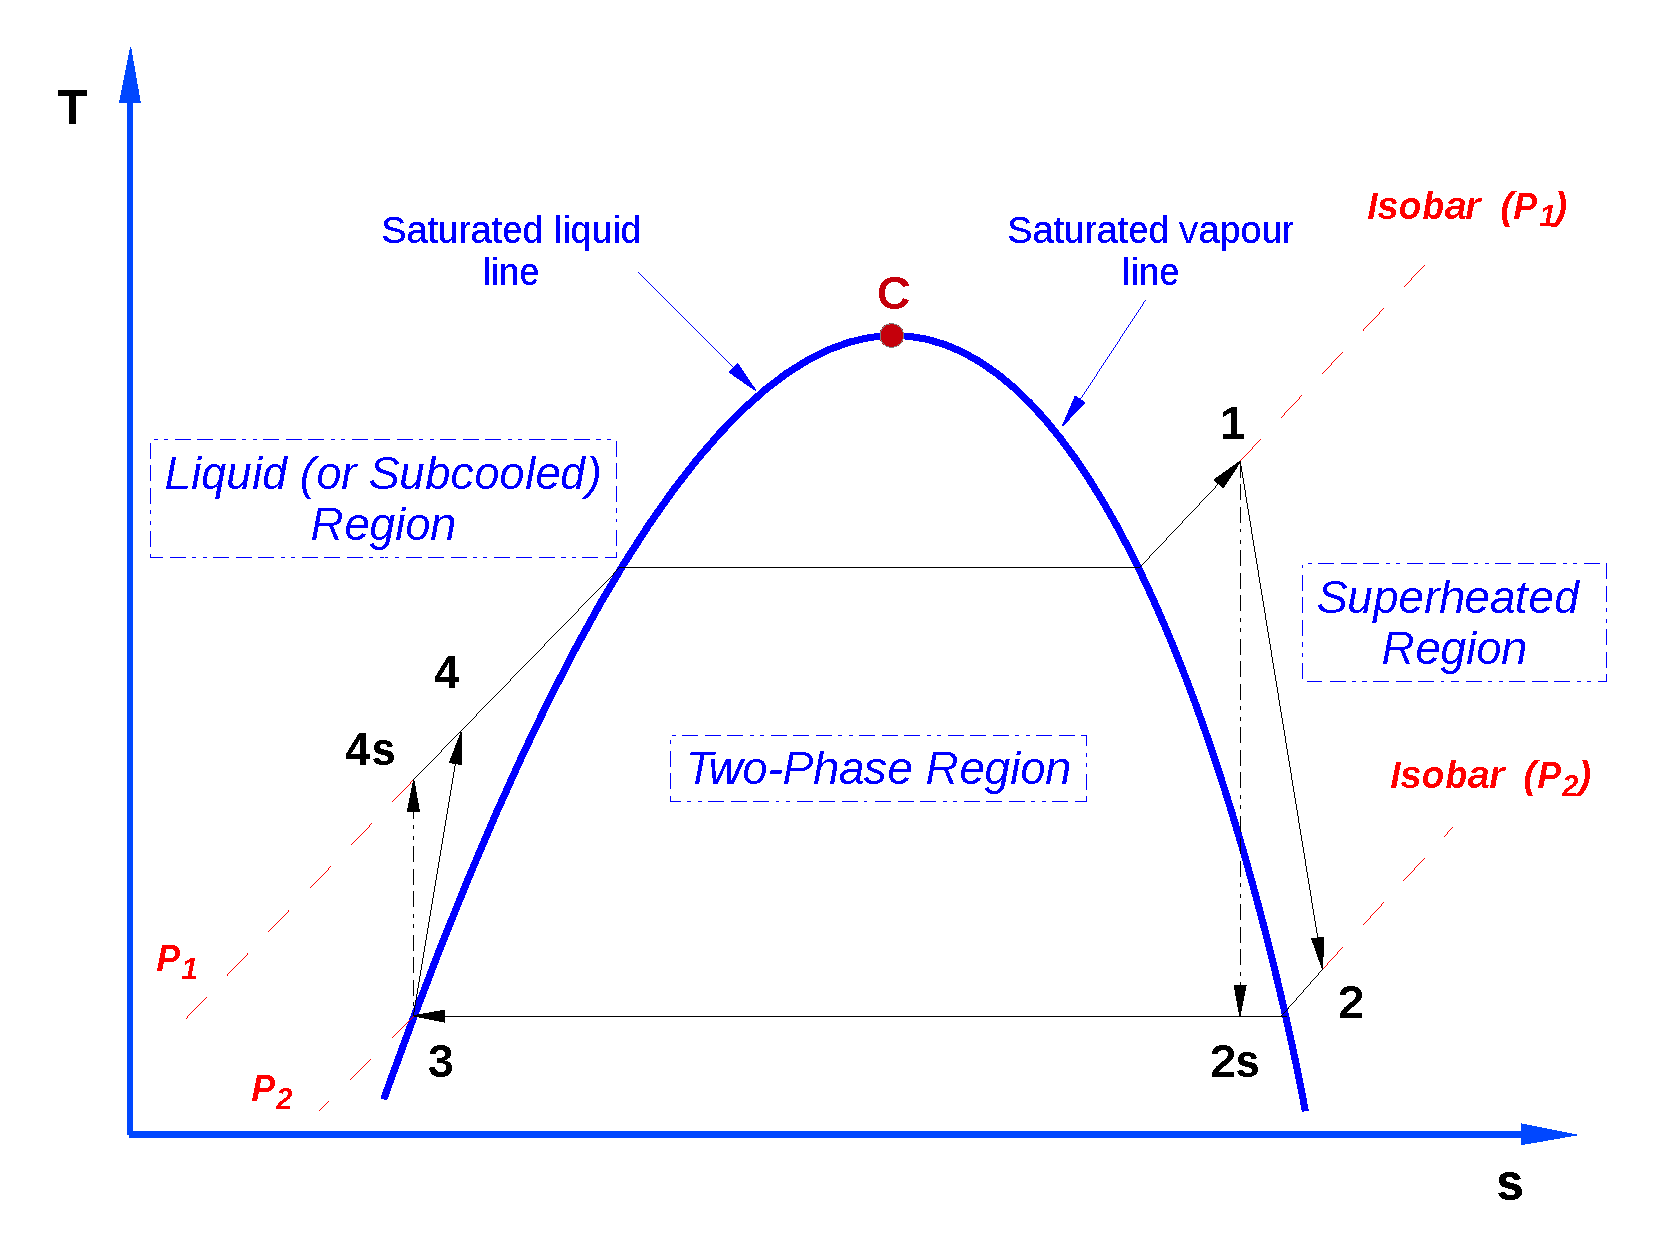
\includegraphics[width=5.5cm,clip]{./Pics/Ideal_Real_Rankine}}
         }
      \end{column}
   \end{columns}
 \normalsize
\end{frame}

%%%
%%% Slide
%%%
\begin{frame}
 \frametitle{Improving the Efficiency of the Rankine Cycles}
   \begin{columns}
      \begin{column}[c]{0.5\linewidth}
         \begin{enumerate}\scriptsize
            \item<1-> The efficiency of the Rankine cycle may be improved by:
              \begin{enumerate}[(a)]\scriptsize
                 \item <1-> Increasing the average temperature at which heat is transferred to the working fluid in the boiler or;
                 \item <1-> Reducing the temperature at which the heat is transferred from the working fluid in the condenser;
              \end{enumerate} 
            \item <2-> This can be achieved with:
              \begin{enumerate}[(a)]\scriptsize
                 \item <2-> Increasing boiler pressure;
                 \item <2-> Use of superheated steam;
                 \item <2-> Reducing condenser pressure.
              \end{enumerate}
            \item <3-> The thermal efficiency can be improved by
              \begin{enumerate}[(a)]\scriptsize
                 \item <3-> Regenerative feed heating;
                 \item <3-> Reheating of steam;
                 \item <3-> Water extraction;
                 \item <3-> Using binary-vapour
              \end{enumerate}
         \end{enumerate}  
      \end{column}
      \begin{column}[c]{0.5\linewidth}
         \visible<2->{\begin{figure}%
           \begin{center}
              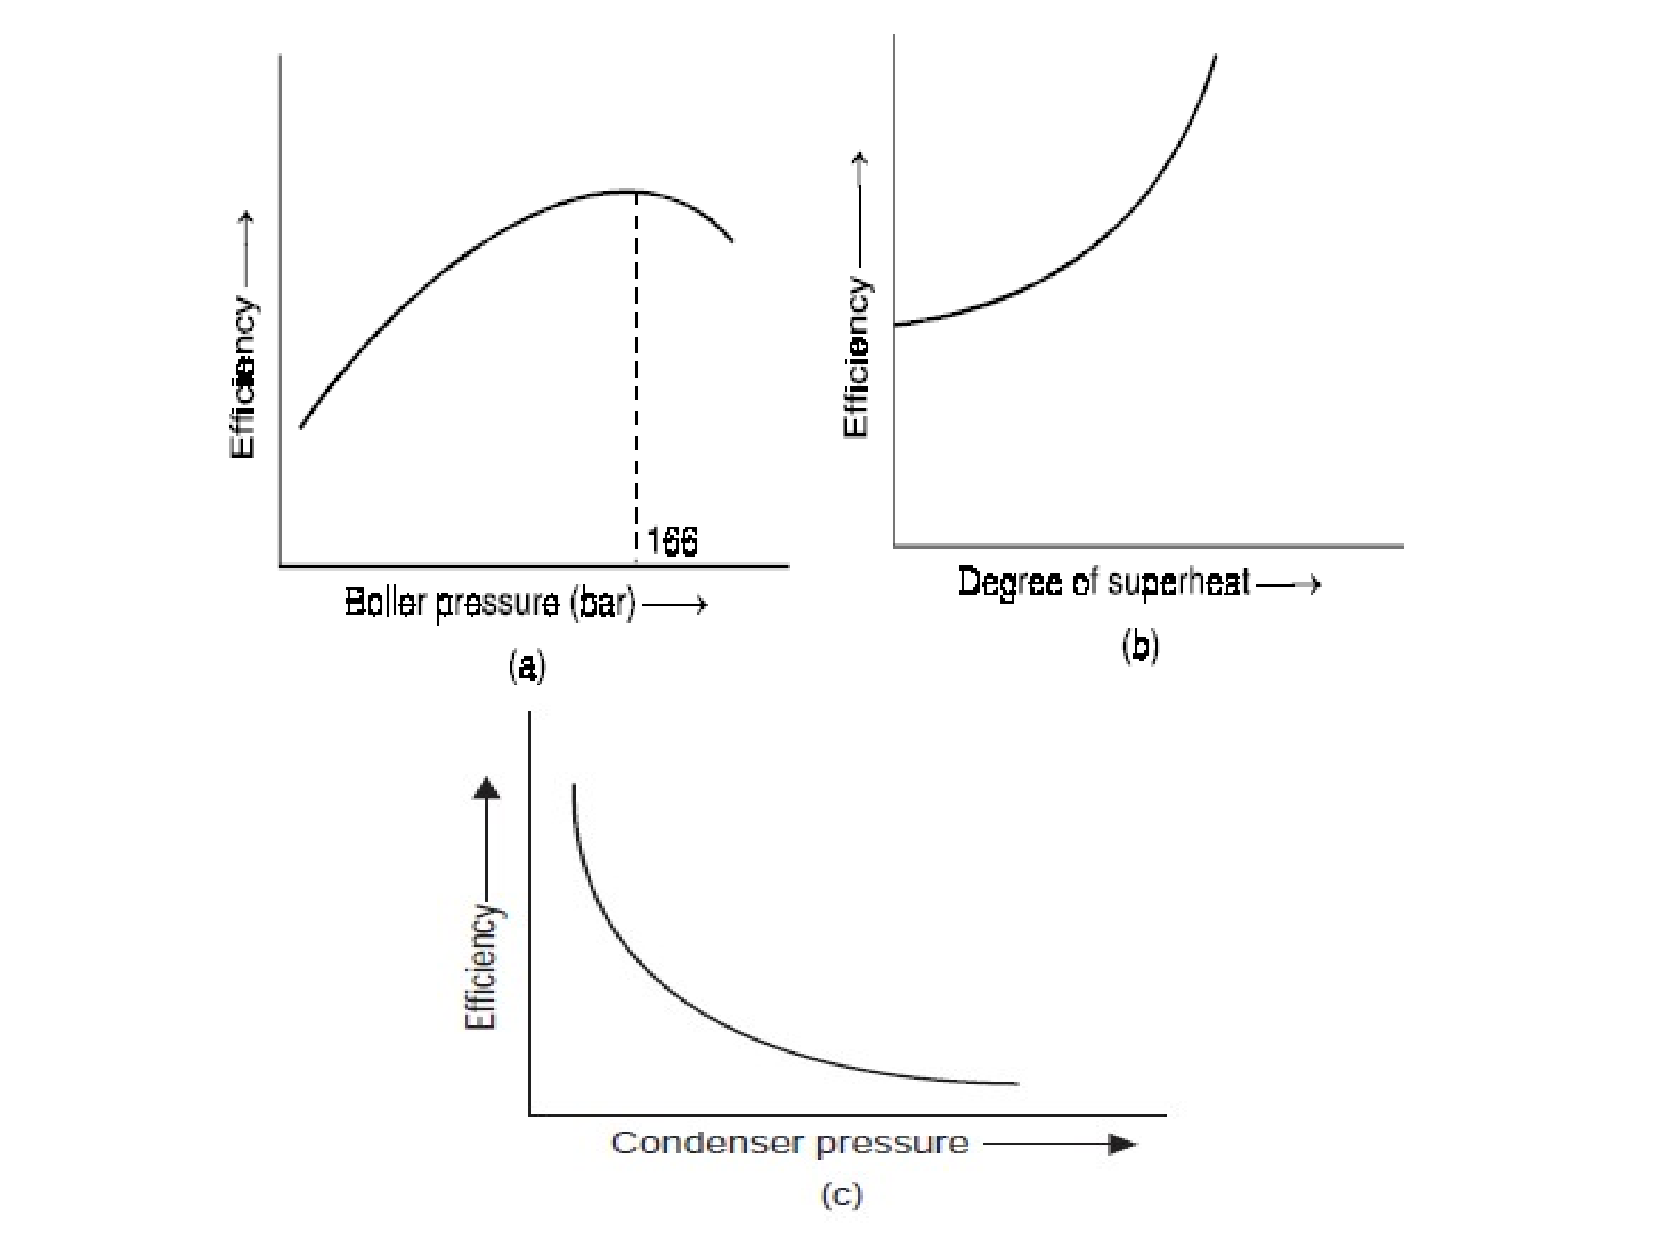
\includegraphics[width=7.cm,clip]{./Pics/Rankine_Improving_Efficiency}
           \end{center}
         \end{figure}}
      \end{column}
   \end{columns}
 \normalsize
\end{frame}

%%%
%%% SUBSECTION
%%%
\subsection{Examples}

%%%
%%% Slide
%%%
\begin{frame}
 \frametitle{Example 1: Carnot and Rankine efficiencies}
 %\scriptsize
    Steam (dry and saturated) is supplied by the boiler at 15 bar and the condenser pressure is 0.4 bar. Calculate the Carnot and Rankine efficiencies of the cycle. Neglect the pump work.
\end{frame}

%%%
%%% Slide
%%%
\begin{frame}
 \frametitle{Example 2: Simple Steam Power Plant}
 \scriptsize
   The table below represents the steps of an idealised steam power plant:
    \begin{center}
     \begin{tabular}{||c | c | c | c | c | c ||}
      \hline\hline
       {\bf Step} & {\bf Location}       & {\bf Pressure}  & {\bf Temperature}     & {\bf Quality /}  &{\bf Velocity}    \\
                  &                      & {\bf (bar)}     &{\bf$\left(^{\circ}\text{C}\right)$}& {\bf State} & {\bf m/s} \\
      \hline\hline
          1       & Inlet to turbine     &   60            &   380                 &  --              &       --         \\
      \hline
          2       & Exit from turbine and&   0.1           &    --                 & 0.9              &  200             \\
                  & inlet to condenser   &                 &                       &                  &                  \\ 
      \hline
          3       & Exit from condenser and&  0.09         &  --                   & Saturated        &  --              \\
                  & inlet to pump        &                 &                       & Liquid           &   --             \\
      \hline
          4       & Exit from pump and   &  70             &   --                  &     --           &   --             \\
                  & inlet to boiler      &                 &                       &                  &                  \\
      \hline 
          5       & Exit from boiler     &  65             &  400                  &      --          &    --            \\
           \hline\hline
     \end{tabular}
    \end{center}
    Assume that the steam mass flow rate leaving the boiler is 10$^{4}$ kg.h$^{-1}$. Sketch the cycle numbering each stage. Calculate:
      \begin{enumerate}[(a)]
         \item Specific enthalpies of all streams;
         \item Power output of the turbine;
         \item Heat transfer per hour in the boiler and condenser;
         \item Mass rate of cooling water circulated (kg/h) in the condenser assuming inlet and outlet fluid temperatures from the condenser of 20$^{\circ}$C and 30$^{\circ}$C;
         \item Diameter of the pipe connecting the turbine with the condenser;
         \item Sketch the $Ts$ diagram, indicating each step of the cycle.
    \end{enumerate}
 \normalsize
\end{frame}

%%%
%%% SECTION
%%%
\section{Modified Rankine Cycles}

\subsection{Reheat Rankine Cycle}

%%%
%%% Slide
%%%
\begin{frame}
 \frametitle{Ideal Reheat Rankine Cycle}
  \begin{columns}
     \begin{column}[c]{0.5\linewidth}
        \begin{enumerate}[(a)] \scriptsize
           \item<1-> Thermal efficiency can be enhanced by increasing the boiler pressure;
           \item<1-> However, this results in higher moisture content in the steam flow which can damage the turbine;
           \item<2-> To overcome this problem we may:
           \begin{enumerate}[(i)] \scriptsize
             \item<2-> Superheat the steam before the turbine: this would improve thermal efficiency of the cycle but the very high temperature may be prohibitive as novel (and more expansive) materials would need to be used;
             \item<2-> \blue{Expand the steam in the turbine in two stages and reheat in between}. This is an improvement on the ideal Rankine cycle as we would add a reheating process between continuous expansion.
           \end{enumerate}
           \item<3-> The \underline{main objective of using superheated steam} is \blue{to avoid excessive moisture in the steam} at the end of the expansion process (maximum moisture content $\sim$ 12$\%$ to avoid turbine blades' damage);
           \item<4-> Advantages of Reheating:
              \begin{enumerate}[(i)]\scriptsize
                 \item<4-> Increase power output from the turbine;
                 \item<4-> Low erosion and corrosion issues;
                 \item<4-> Improvement of the thermal efficiency of the turbines.
              \end{enumerate}
        \end{enumerate}
     \end{column}
     \begin{column}[c]{0.5\linewidth} 
        \visible<2->{\begin{figure}%
           \begin{center}
             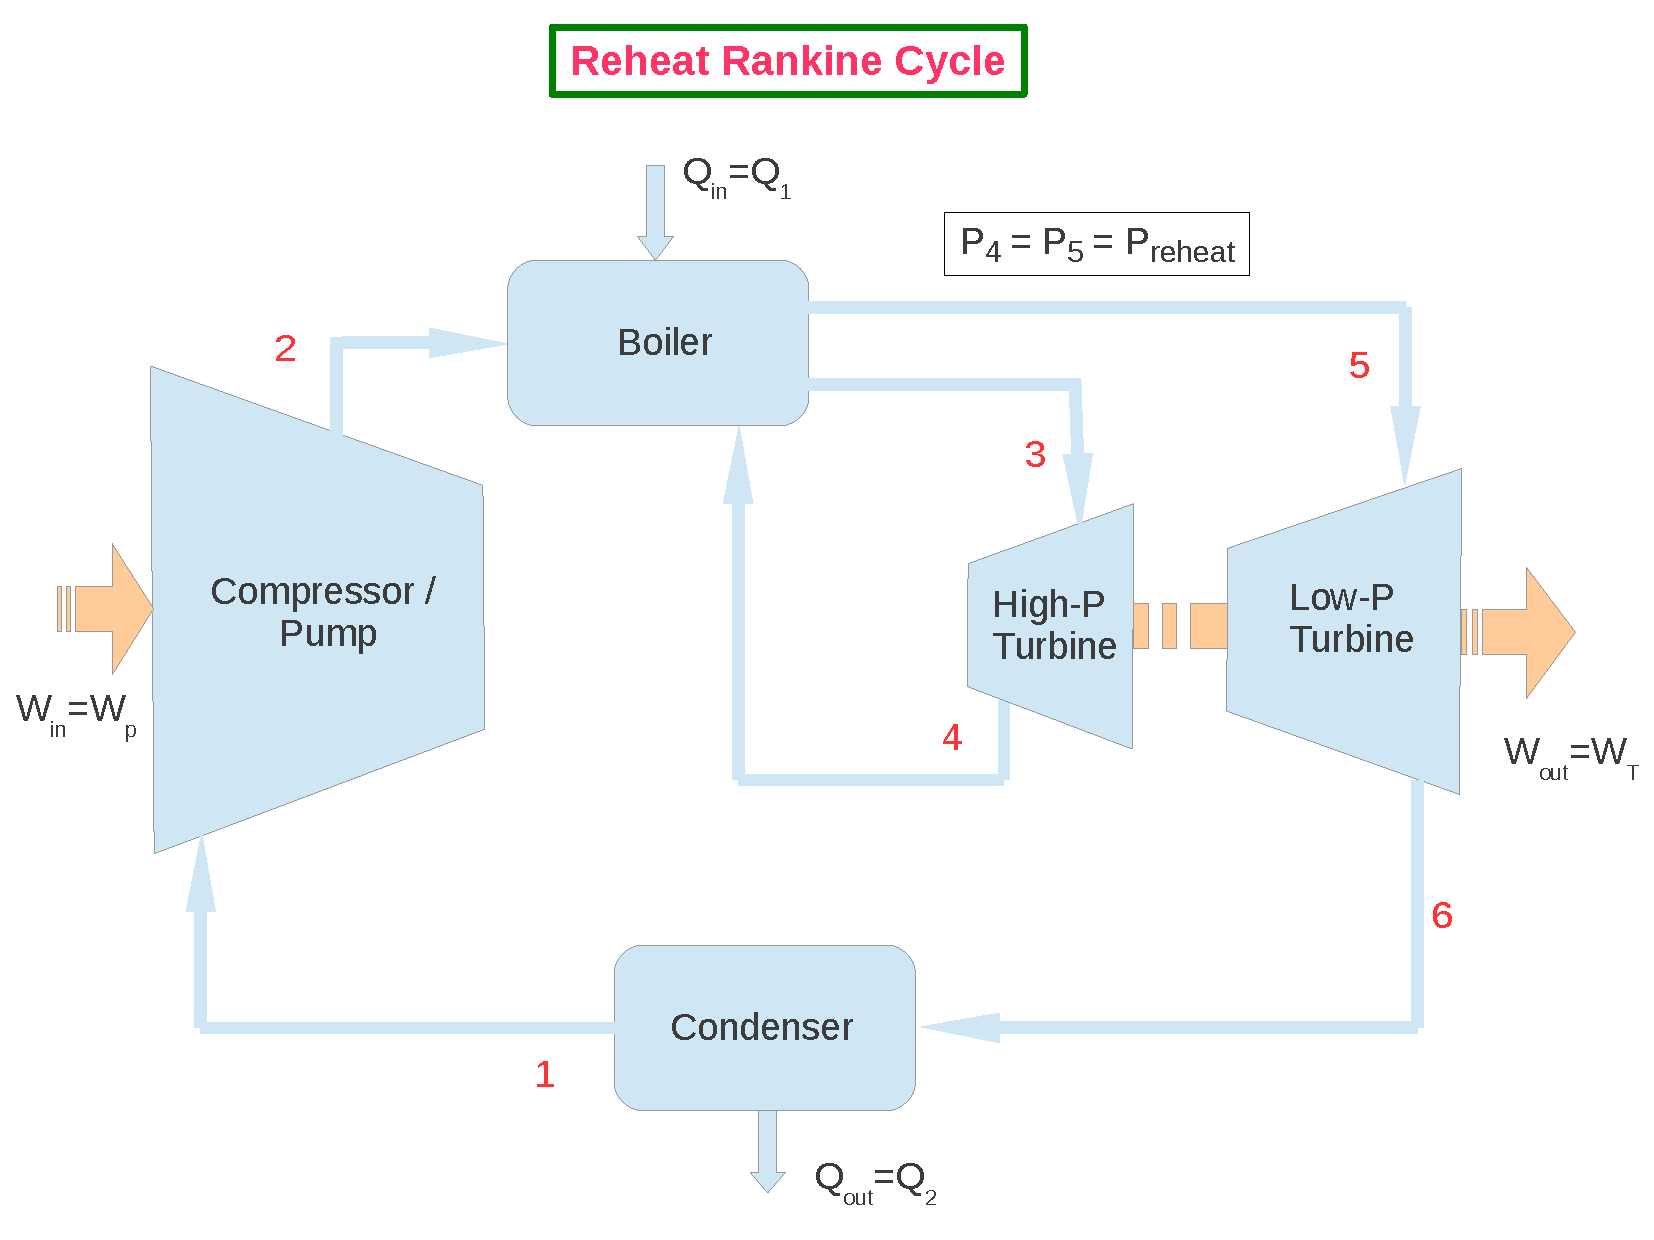
\includegraphics[width=6.25cm,clip]{./Pics/Reheat_Rankine_Cycle}
           \end{center}
        \end{figure}} 
        \begin{enumerate}[(a)]\scriptsize\setcounter{enumi}{5}
           \item<5-> Disadvantages of Reheating:
              \begin{enumerate}[(i)]\scriptsize
                 \item<5->Reheating requires more maintenance;
                 \item<5->Enhancement of thermal efficiency may not be enough to match the larger costs associated with reheating the steam.
              \end{enumerate}
        \end{enumerate}
     \end{column}
  \end{columns}
 \normalsize
\end{frame}


%%%
%%% Slide
%%%
\begin{frame}
 \frametitle{Ideal Reheat Rankine Cycle}
  \begin{columns}
     \begin{column}[c]{0.5\linewidth} 
       \begin{center}
          \begin{figure}
             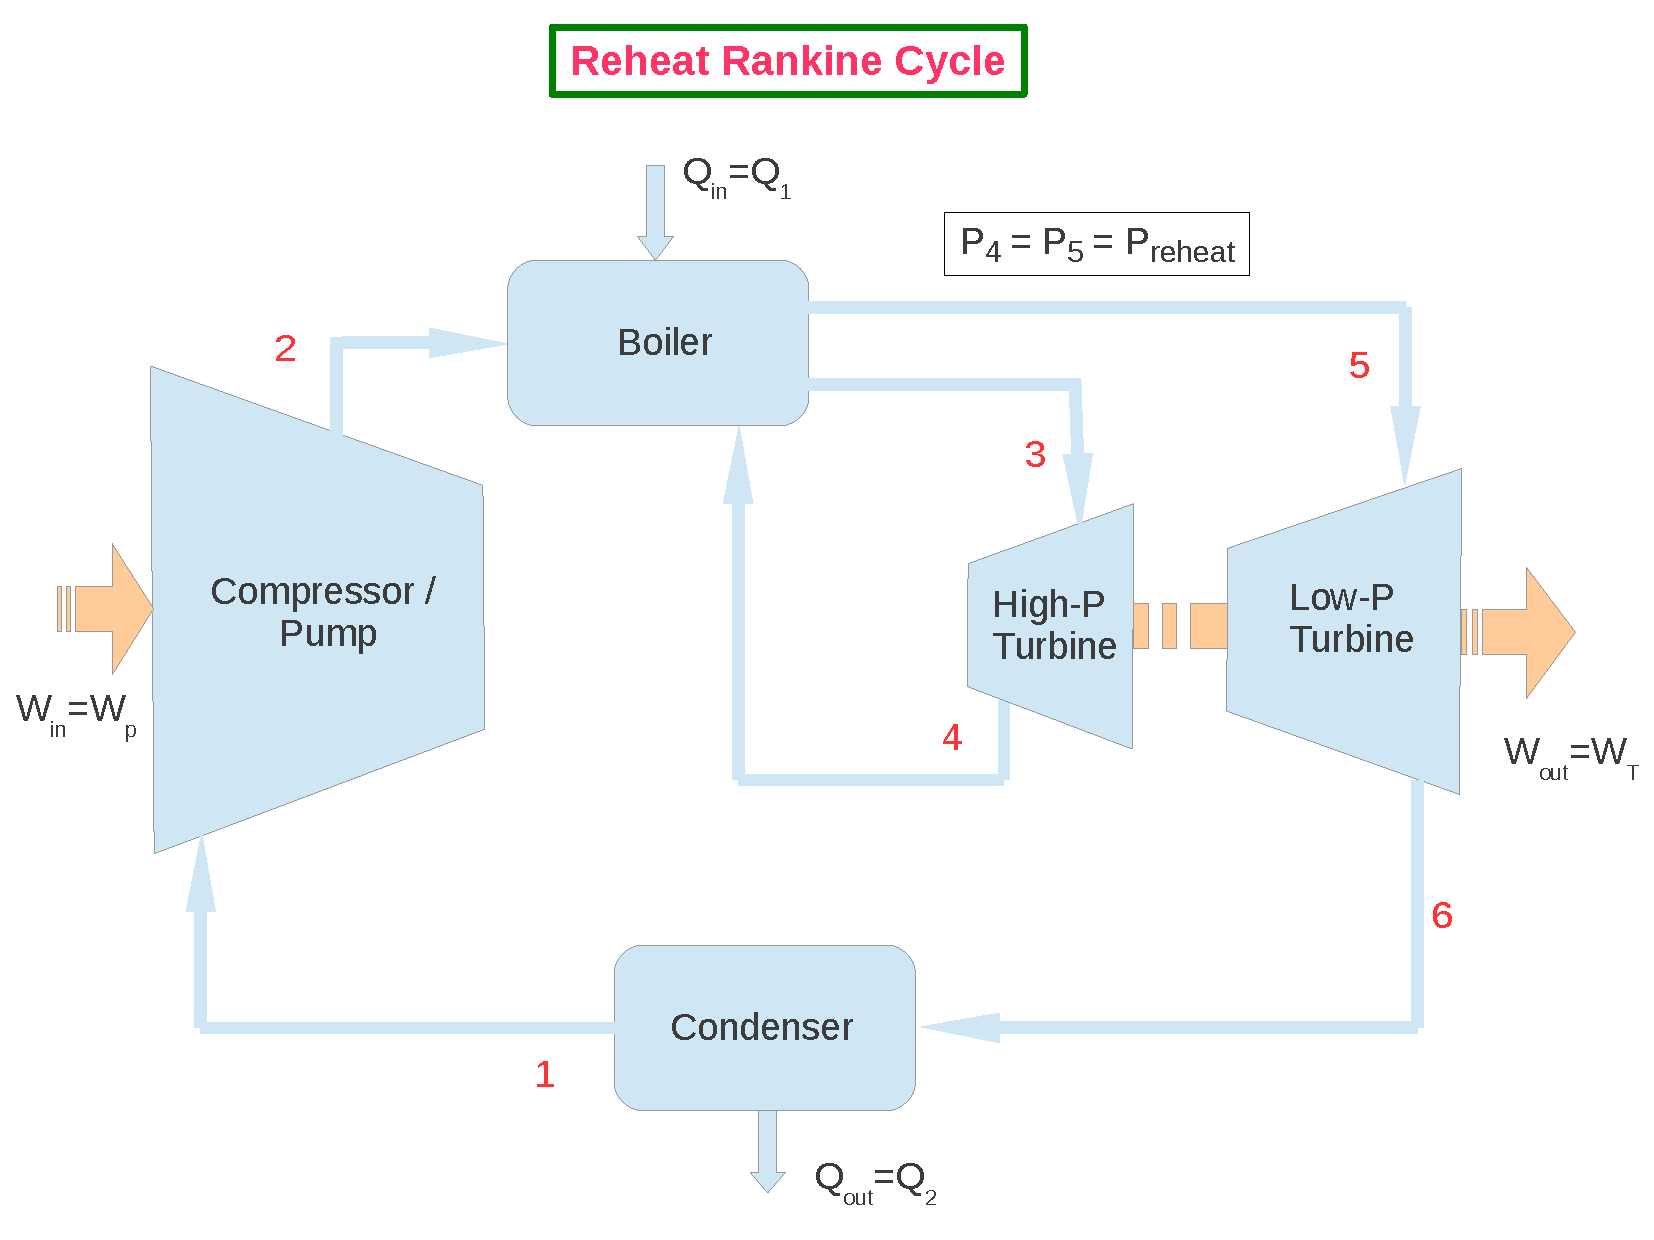
\includegraphics[width=6.25cm,clip]{./Pics/Reheat_Rankine_Cycle}
          \end{figure}
       \end{center}
       \begin{enumerate}[(a)] \scriptsize\setcounter{enumi}{6}
          \item<1-> Total heat input: 
              \visible<1->{\begin{eqnarray}
                  \blue{Q_{\text{total}}}&=& Q_{\text{primary}} + Q_{\text{reheat}} \nonumber \\
                                    &=& \blue{\left(h_{1}-h_{6}\right)+\left(h_{3}-h_{2}\right)}
              \end{eqnarray}}
       \end{enumerate}
     \end{column}
     \begin{column}[c]{0.5\linewidth}
       \begin{center}
          \begin{figure}
             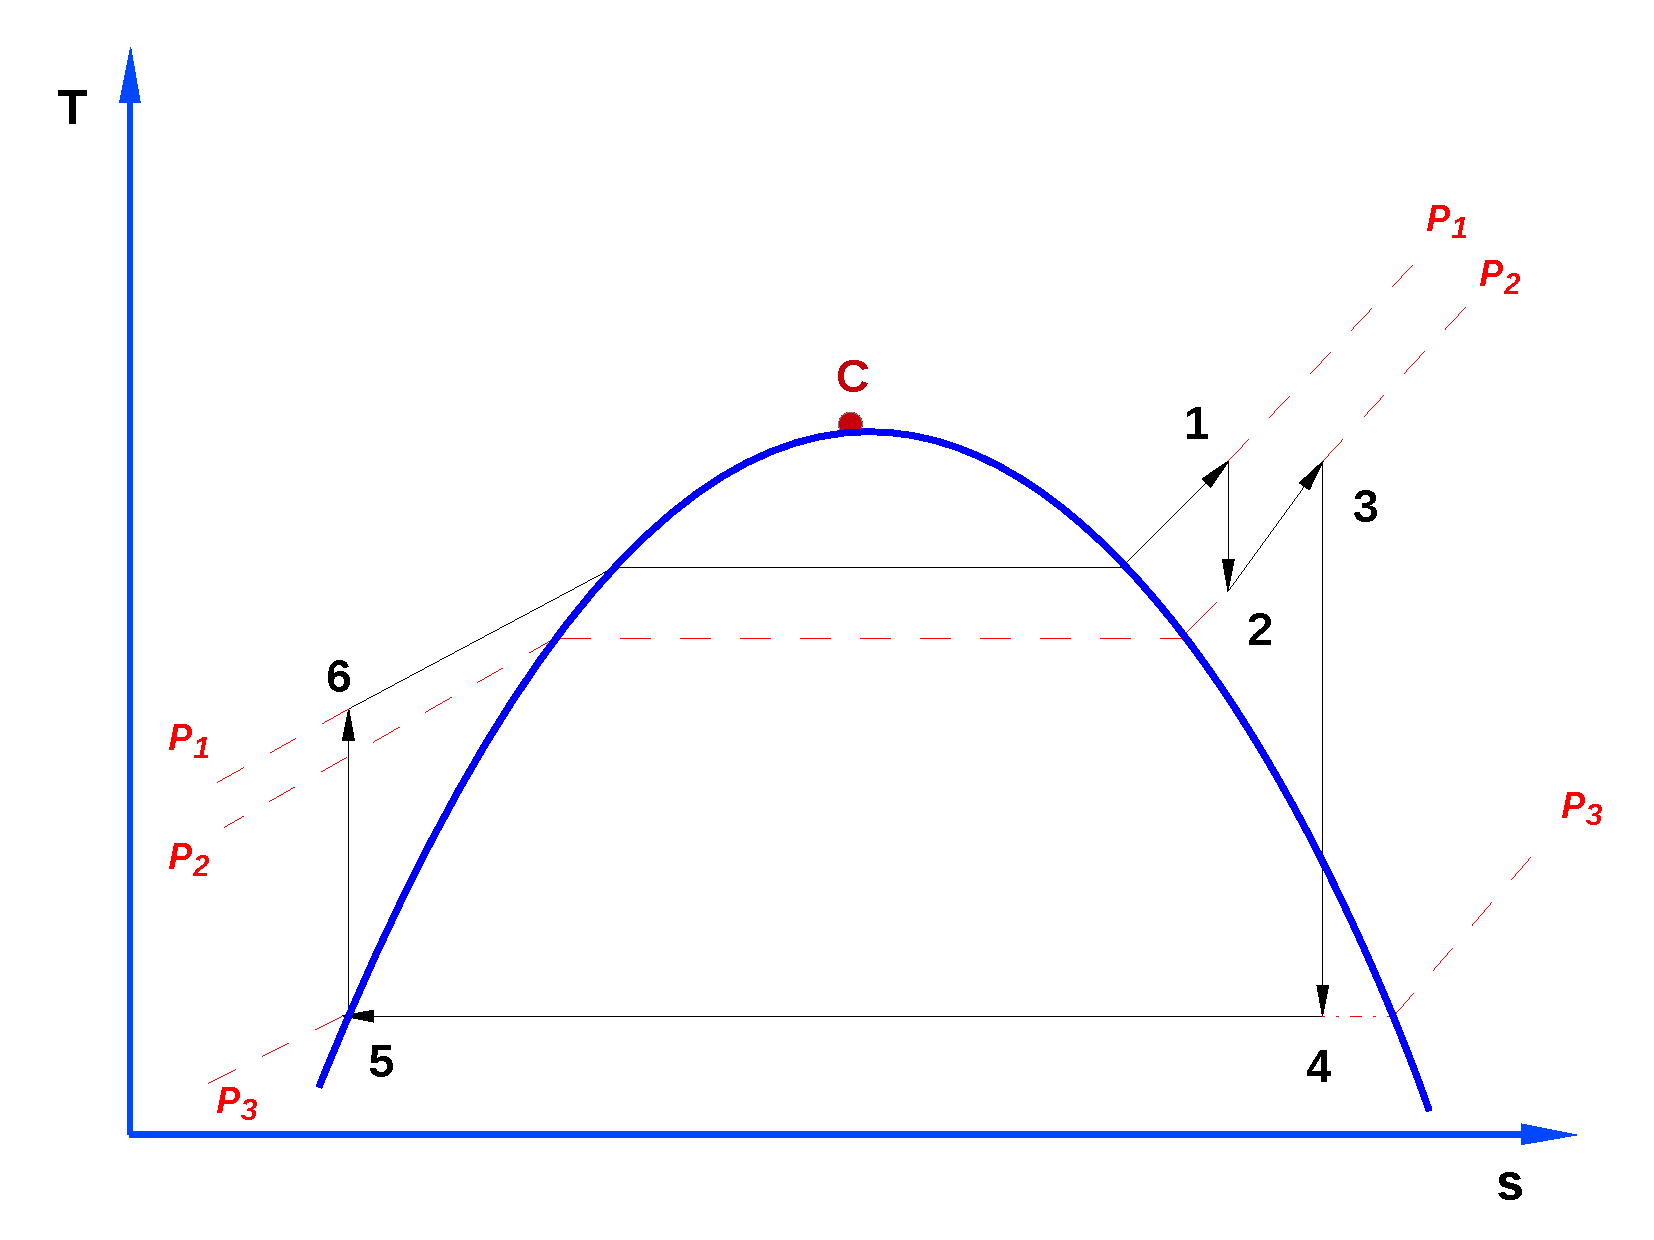
\includegraphics[width=6.25cm,clip]{./Pics/Reheat_Rankine_Cycle_Diagram2}
          \end{figure}
       \end{center}
       \begin{enumerate}[(a)] \scriptsize\setcounter{enumi}{7}
          \item<2-> Total turbine work output:
              \visible<2->{\begin{eqnarray}
                  \blue{W_{\text{turbine}}^{\text{total}}} &=& W_{\text{turbine}}^{\text{high-P}} + W_{\text{turbine}}^{\text{low-P}} \nonumber \\
                                                      &=& \blue{\left(h_{2}-h_{1}\right)+\left(h_{4}-h_{3}\right)}
              \end{eqnarray}}
       \end{enumerate}
     \end{column}
  \end{columns}
 \normalsize
\end{frame}


\end{document}
 
